% Compile with XeLaTeX -> BibTeX -> XeLaTeX -> XeLaTeX.
% Text is generated from ../THESIS_DRAFT.md; do not edit content/*.tex by hand.
\documentclass[fontsize=13pt,paper=a4,DIV=calc,oneside,open=any,headings=normal,numbers=noenddot]{scrbook}
\usepackage{lmodern}
\usepackage{fontspec}
\IfFontExistsTF{Times New Roman}{\setmainfont{Times New Roman}}{\setmainfont{TeX Gyre Termes}}
\setsansfont{TeX Gyre Heros}
\setmonofont{Latin Modern Mono}[Scale=MatchLowercase]
\usepackage[a4paper,top=2.5cm,bottom=3cm,left=3cm,right=2cm,headheight=21pt]{geometry}
\usepackage{amsmath,amssymb,graphicx,booktabs,longtable,array}
\usepackage{setspace,indentfirst,caption,scrlayer-scrpage,xurl}
\usepackage[unicode,hidelinks,breaklinks=true]{hyperref}
\usepackage{fvextra}
\usepackage{tikz}
\usetikzlibrary{calc}
\setstretch{1.3}
\setlength{\parindent}{1cm}
\setlength{\parskip}{6pt}
\setlength{\emergencystretch}{2em}
\setlength{\LTpre}{8pt plus 2pt minus 2pt}
\setlength{\LTpost}{8pt plus 2pt minus 2pt}
\setcounter{secnumdepth}{2}
\setcounter{tocdepth}{2}
\setkomafont{disposition}{\normalfont\bfseries}
\setkomafont{pageheadfoot}{\normalfont}
\setlength{\footheight}{21pt}
\RedeclareSectionCommand[beforeskip=0pt,afterskip=22pt]{chapter}
\RedeclareSectionCommand[beforeskip=15pt plus 3pt minus 2pt,afterskip=8pt plus 2pt,afterindent=true]{section}
\AddToHook{begindocument/end}{%
  \renewcommand{\chaptername}{Chương}%
  \renewcommand{\contentsname}{Mục lục}%
  \renewcommand{\listfigurename}{Danh mục hình}%
  \renewcommand{\listtablename}{Danh mục bảng}%
  \renewcommand{\bibname}{Tài liệu tham khảo}%
  \renewcommand{\appendixname}{Phụ lục}%
}
\captionsetup[figure]{name=Hình,position=bottom,labelfont=bf,labelsep=period}
\captionsetup[table]{name=Bảng,position=top,labelfont=bf,labelsep=period}
\clearpairofpagestyles
\cfoot*{\pagemark}
\newcommand{\thesistitle}{Nâng cao khả năng xử lý tác vụ chuỗi dài cho mô hình VLA trong điều khiển Robot}
\hypersetup{pdftitle={\thesistitle},pdfauthor={Lưu Quang Linh},pdfsubject={Khóa luận về bộ nhớ sự kiện thị giác cho mô hình VLA},pdflang={vi-VN}}

\begin{document}
\pagenumbering{Roman}
% Metadata confirmed by the student; no signature is generated.
\newcommand{\coverframe}{%
  \begin{tikzpicture}[remember picture,overlay]
    \draw[line width=2pt] ($(current page.north west)+(2cm,-2cm)$)
      rectangle ($(current page.south east)+(-1.5cm,1.8cm)$);
    \draw[line width=.7pt] ($(current page.north west)+(2.15cm,-2.15cm)$)
      rectangle ($(current page.south east)+(-1.65cm,1.95cm)$);
  \end{tikzpicture}}
\begin{titlepage}
\thispagestyle{empty}\coverframe
\begin{center}
{\bfseries ĐẠI HỌC QUỐC GIA HÀ NỘI\\TRƯỜNG ĐẠI HỌC CÔNG NGHỆ\par}
\vspace{1cm}

\includegraphics[width=2.4cm]{assets/UET.png}\par
\vspace{1cm}
{\Large\bfseries LƯU QUANG LINH\par}
\vspace{1.5cm}
{\fontsize{18}{25}\selectfont\bfseries\MakeUppercase{\thesistitle}\par}
\vspace{1.8cm}
{\bfseries KHÓA LUẬN TỐT NGHIỆP ĐẠI HỌC HỆ CHÍNH QUY\par}
\vspace{.3cm}
{\bfseries Ngành: Trí tuệ nhân tạo\par}
\vfill
{\bfseries HÀ NỘI -- 2026\par}
\end{center}
\end{titlepage}

\begin{titlepage}
\thispagestyle{empty}\coverframe
\begin{center}
{\bfseries ĐẠI HỌC QUỐC GIA HÀ NỘI\\TRƯỜNG ĐẠI HỌC CÔNG NGHỆ\par}
\vspace{1.3cm}
{\Large\bfseries LƯU QUANG LINH\par}
{Mã sinh viên: 23020392\quad Lớp: K68A-AI2\par}
\vspace{1.3cm}
{\fontsize{18}{25}\selectfont\bfseries\MakeUppercase{\thesistitle}\par}
\vspace{1.6cm}
{\bfseries KHÓA LUẬN TỐT NGHIỆP ĐẠI HỌC HỆ CHÍNH QUY\par}
{\bfseries Ngành: Trí tuệ nhân tạo\par}
\vspace{1.8cm}
\begin{minipage}{.92\textwidth}
\textbf{Cán bộ hướng dẫn:} PGS.TS. Nguyễn Việt Hà\par
\textbf{Cán bộ đồng hướng dẫn:} PGS.TS. Hoàng Văn Xiêm\par
\end{minipage}
\vfill
{\bfseries HÀ NỘI -- 2026\par}
\end{center}
\end{titlepage}

\pagestyle{empty}
\chapter*{Lời cảm ơn}
\thispagestyle{empty}

Lời đầu tiên, em xin được gửi lời cảm ơn chân thành và sâu sắc nhất tới \textbf{PGS. TS. Nguyễn Việt Hà} và \textbf{PGS. TS. Hoàng Văn Xiêm}, những người thầy đã luôn tận tâm định hướng nghiên cứu, trực tiếp chỉ bảo và tạo mọi điều kiện thuận lợi nhất cho em trong suốt quá trình thực hiện khóa luận tốt nghiệp này.

Em cũng xin gửi lời cảm ơn tới các thầy cô giáo tại Trường Đại học Công nghệ, Đại học Quốc gia Hà Nội, đặc biệt là cô Nguyễn Thị Thùy Linh đã truyền đạt những kiến thức quý báu và nền tảng chuyên môn vững chắc cho em trong suốt những năm học tập và nghiên cứu vừa qua của em.

Cuối cùng, con xin gửi lời cảm ơn sâu sắc tới gia đình và bạn bè, những người đã luôn ở bên động viên, ủng hộ và là chỗ dựa tinh thần vững chắc để con - em hoàn thành tốt khóa luận này.

\vspace{1.5cm}
\begin{flushright}
\begin{tabular}{c}
\textit{Hà Nội, tháng 11 năm 2026} \\
\textbf{Sinh viên thực hiện} \\
\vspace{2cm} \\
\textbf{Lưu Quang Linh}
\end{tabular}
\end{flushright}

% Generated from THESIS_DRAFT.md.
\chapter*{Tóm tắt}
\thispagestyle{empty}

Trong thao tác robot ở chuỗi tác vụ dài, các quan sát cảm biến robot thu được sau khi hoàn tất một chu kỳ thao tác thường tương tự với quan sát ban đầu, trong khi quyết định tiếp tục hay dừng chuỗi hành động lại phụ thuộc vào số chu kỳ và mốc tiến độ đã hoàn tất. Nhằm giải quyết hiện tượng này, khóa luận đề xuất một kiến trúc bộ nhớ theo sự kiện có khả năng biểu diễn mạch lạc thông tin tiến độ và hỗ trợ các mô hình thị giác - ngôn ngữ - hành động (VLA) thực hiện các tác vụ chuỗi cần bộ nhớ. Nghiên cứu tập trung giải quyết bài toán trên bộ tiêu chuẩn thao tác chuỗi dài, đặc biệt hướng tới việc nâng cao năng lực cho các mô hình VLA nhỏ gọn vốn chịu nhiều ràng buộc nghiêm ngặt về độ dài ngữ cảnh và tài nguyên tính toán.

Phương pháp đề xuất biểu diễn tiến độ bằng cách xác định trạng thái vật thể và robot hiện tại, mô tả lại sự kiện đã xảy ra một cách thích ứng với tác vụ và quan sát. Mỗi sự kiện đều được lưu vết đầy đủ bằng chứng và thời điểm để sử dụng nhằm đảm bảo độ tin cậy và tính nhân quả. Ngay cả khi lịch sử chưa được quan sát đầy đủ, bộ nhớ vẫn có thể biểu diễn tiến độ một cách thích ứng. Hai tính chất của hệ bộ nhớ đề xuất được chứng minh trong phạm vi khóa luận bao gồm: Bộ đếm và ghi nhận sự kiện chỉ thay đổi khi xuất hiện một sự kiện kích hoạt hợp lệ; Nội dung cấp cho chính sách tại một thời điểm chỉ phụ thuộc vào dữ liệu sẵn có đến thời điểm đó. Bộ nhớ sự kiện này sau đó được chiếu thành một bản tóm tắt ngôn ngữ tự nhiên gọn nhẹ, đưa vào đầu vào điều kiện hóa của mô hình VLA với phần sinh hành động đã được huấn luyện thích ứng.

Hiệu quả của phương pháp được kiểm chứng thông qua các thực nghiệm trên Bộ tiêu chuẩn đánh giá khả năng học tập suốt đời của robot LIBERO và Bộ tiêu chuẩn thao tác chuỗi dài LIBERO-Mem, bao gồm cả đánh giá về năng lực tri giác và đánh giá điều khiển vòng kín trên mô hình VLA. Kết quả cho thấy bộ theo dõi thị giác có khả năng phát hiện và đồng bộ chính xác các mốc sự kiện vật lý từ dòng quan sát thô mà không cần tiếp cận trạng thái đặc quyền của môi trường mô phỏng. Khi tích hợp vào vòng điều khiển kín, thông tin bộ nhớ sự kiện cung cấp tín hiệu tiến độ then chốt giúp mô hình phân giải tính đa nghĩa của quan sát thị giác, định hướng chuỗi hành động đúng tiến độ và ngăn ngừa các lỗi lặp lại chu kỳ hoặc kết thúc sớm. Đồng thời, các phân tích chuyên sâu làm sáng tỏ mối quan hệ phụ thuộc giữa độ trễ tích lũy bằng chứng, độ hoàn thiện của lịch sử quan sát và độ ổn định của chính sách điều khiển. Nghiên cứu qua đó xác lập một khung phương pháp luận có tính khả kiểm cao, đặt nền tảng vững chắc cho việc mở rộng kiến trúc bộ nhớ sự kiện - bằng chứng cho các bài toán thao tác đa bước phức tạp trên các mô hình robot học sâu.

\textbf{Từ khóa:} mô hình thị giác - ngôn ngữ - hành động, SmolVLA, bộ nhớ sự kiện, quan sát một phần, thao tác robot.


\chapter*{Lời cam đoan}
\thispagestyle{empty}

Tôi xin cam đoan đây là công trình nghiên cứu của chính tôi dưới sự hướng dẫn khoa học của PGS. TS. Nguyễn Việt Hà và PGS. TS. Hoàng Văn Xiêm. 

Các kết quả nghiên cứu, phân tích và số liệu được trình bày trong khóa luận là hoàn toàn trung thực, khách quan và chưa từng được công bố trong bất kỳ công trình nào khác. Mọi thông tin, dữ liệu, mã nguồn và tài liệu tham khảo được kế thừa từ các công trình nghiên cứu khác đều đã được trích dẫn và ghi nhận nguồn gốc đầy đủ, rõ ràng theo đúng các quy định về liêm chính học thuật.

\vspace{1.5cm}
\begin{flushright}
\begin{tabular}{c}
\textit{Hà Nội, tháng 11 năm 2026} \\
\textbf{Sinh viên cam đoan} \\
\vspace{2cm} \\
\textbf{Lưu Quang Linh}
\end{tabular}
\end{flushright}

\frontmatter
\pagestyle{scrheadings}
\tableofcontents
\listoffigures
\listoftables
\addchap{Danh mục ký hiệu và chữ viết tắt}
\begin{longtable}{p{.20\textwidth}p{.74\textwidth}}
VLA & Mô hình thị giác--ngôn ngữ--hành động\\
VLM & Mô hình thị giác--ngôn ngữ\\
POMDP & Quá trình quyết định Markov quan sát một phần\\
FSM & Máy trạng thái hữu hạn\\
LoRA & Thích ứng hạng thấp\\
SFT & Tinh chỉnh có giám sát\\
RQ & Câu hỏi nghiên cứu\\
SR & Tỷ lệ lượt thực thi thành công\\
SCR & Tỷ lệ mục tiêu thành phần đã hoàn thành\\
RGB & Đỏ--lục--lam, biểu diễn ảnh màu\\
IoU & Giao trên hợp giữa hai hộp giới hạn\\
T1, T3 & Tác vụ nhấc và đặt lại bát một lần và ba lần\\
B0 & Chính sách SmolVLA gốc\\
F0 & Đối chứng thích ứng với cùng dữ liệu và ngân sách, bỏ đầu vào bộ nhớ\\
F1 & Chính sách SmolVLA với adapter huấn luyện có bộ nhớ\\
F1-off & Chính sách F1 với bộ nhớ bị tắt trong suy luận\\
$H$ & Số bước trong chuỗi hành động dự đoán\\
$s$ & Số hành động thực thi trước lần truy vấn tiếp theo\\
$m_t$ & Trạng thái bộ nhớ khả dụng tại bước $t$\\
$o_t$ & Quan sát chính sách được phép sử dụng\\
$x_t$ & Trạng thái đầy đủ của bài toán tại bước $t$\\
$h_t$ & Lịch sử quan sát--hành động đến bước $t$\\
$N$ & Số chu kỳ theo yêu cầu của tác vụ\\
$z_t$ & Số chu kỳ đã hoàn tất theo định nghĩa tác vụ tại bước $t$\\
$\hat z_t$ & Số chu kỳ bộ ghi đã xác nhận đến bước $t$\\
$\tau_j,\upsilon_j$ & Thời điểm ước lượng sự kiện xảy ra và thời điểm bằng chứng khả dụng\\
\end{longtable}
\mainmatter
% Generated from THESIS_DRAFT.md.
\chapter{Mở đầu}

\section{Bối cảnh nghiên cứu}

Mô hình thị giác–ngôn ngữ–hành động, gọi tắt là VLA, kết nối quan sát hình ảnh, chỉ dẫn ngôn ngữ và hành động điều khiển robot trong một policy. Khả năng tái sử dụng biểu diễn đã học từ dữ liệu thị giác và ngôn ngữ làm cho hướng tiếp cận này phù hợp với các tác vụ thao tác được mô tả bằng lời. SmolVLA là một đại diện hướng đến mô hình có chi phí triển khai thấp hơn, sử dụng một backbone thị giác–ngôn ngữ cùng action expert để sinh chuỗi hành động \cite{smolvla2025}. Tuy nhiên, một policy có thể thực hiện thao tác đơn lẻ vẫn chưa chắc xử lý được nhiệm vụ mà quyết định tiếp theo phụ thuộc vào lịch sử.

Xét yêu cầu nhấc một chiếc bát khỏi đĩa rồi đặt lại đúng ba lần. Sau mỗi lần đặt lại, hình ảnh bát trên đĩa có thể gần giống ban đầu. Nếu chỉ quan sát cảnh hiện tại, hệ thống khó phân biệt đã hoàn thành một, hai hay ba lần. Hành động cần thực hiện vì thế không chỉ phụ thuộc vị trí hiện tại của bát mà còn phụ thuộc những lần tương tác trước đó. Ví dụ này cũng chỉ ra rằng chiều dài trajectory và mức cần thiết của memory là hai thuộc tính khác nhau: một nhiệm vụ dài có thể bộc lộ tiến độ ngay trong cảnh, trong khi một nhiệm vụ lặp ngắn hơn có thể cần lịch sử để phân biệt các tình huống.

Các nghiên cứu gần đây đã khảo sát nhiều biểu diễn memory. MEM phối hợp lịch sử ảnh ngắn với tóm tắt ngôn ngữ dài, còn MemoryVLA lưu và truy xuất các biểu diễn perceptual và cognitive trong một memory bank \cite{mem2026,memoryvla2026}. LIBERO-Mem xây dựng các tình huống thao tác có thông tin quan trọng gắn với lịch sử của thực thể \cite{liberomem2025}. Những công trình này tạo động lực nghiên cứu, đồng thời cho thấy không thể đánh giá memory chỉ bằng việc thêm một chuỗi văn bản vào instruction rồi quan sát một vài rollout.

\section{Bài toán đặt ra}

Khóa luận nghiên cứu cách bổ sung một bộ nhớ sự kiện bên ngoài SmolVLA. Bộ nhớ phải được xây dựng từ quan sát được phép sử dụng, giữ thông tin có ích qua thời gian và tạo đầu vào phù hợp cho policy. Hai yêu cầu cần được giải quyết đồng thời là tính đúng đắn của thông tin được ghi và khả năng policy khai thác thông tin đó. Một hệ thống ghi nhiều sự kiện nhưng thường nhầm lẫn không đương nhiên tốt hơn hệ thống có khả năng từ chối xác nhận khi thiếu bằng chứng.

Trong phạm vi hiện tại, bài toán được thu hẹp vào quan hệ giữa một chiếc bát và đĩa gốc của nó. Hệ thống theo dõi các lần bát rời đĩa và quay lại. T1 yêu cầu một lần nhấc–đặt lại; T3 yêu cầu ba lần. Đây là tập con của hướng nghiên cứu về thao tác có lịch sử thực thể, chưa đại diện cho memory nhiều vật thể, quan hệ chứa, thứ tự tương tác phức tạp hoặc chuyển giao sang robot thật.

Một khó khăn độc lập với thiết kế memory là tính hợp lệ của phép đo. Policy, simulator, dữ liệu demonstration, bộ tiền xử lý và bộ chấm điểm phải có nguồn gốc rõ ràng. Nếu quy ước ảnh hoặc điều kiện kết thúc khác nhau, chênh lệch success có thể phản ánh thay đổi của đường thực nghiệm thay vì thông tin lịch sử. Vì vậy, xây dựng một phép so sánh có thể kiểm tra lại là một phần của phương pháp nghiên cứu.

Có thể mô tả bài toán ở mức trừu tượng như sau. Tại thời điểm $t$, môi trường có trạng thái đầy đủ $x_t$, nhưng policy chỉ nhận quan sát được cho phép $o_t$, instruction $ell$ và snapshot lịch sử $m_t$. Mục tiêu của task là số chu kỳ cần hoàn thành $N\in\{1,3\}$. Gọi $z_t$ là số chu kỳ vật lý đã thực hiện và $\hat z_t$ là số chu kỳ writer đã xác nhận. Hai đại lượng này không đồng nhất: $z_t$ thuộc trạng thái mô phỏng và evaluator, còn $\hat z_t$ là ước lượng từ bằng chứng RGB có thể thiếu hoặc sai.

Tại mỗi lần truy vấn, policy nhận chuỗi điều kiện $c_t=R(\ell,m_t)$ và sinh một action chunk $A_t$. Yêu cầu thiết kế là duy trì một bộ nhớ có ích cho quyết định nhưng tuân theo ràng buộc thông tin và giao diện:

\begin{equation}
\begin{aligned}
m_t &= U(m_{t-1},o_t,a_{t-1}),\\
A_t &\sim \pi_{\theta,\phi}(\cdot\mid o_t,c_t),\\
\operatorname{Tok}(\ell\oplus R(\ell,m_t)) &\le 48.
\end{aligned}
\end{equation}

Ở đây $a_{t-1}$ là action đã thực thi trước quan sát hiện tại; $\oplus$ biểu thị phép ghép instruction với memory theo đúng quy ước tiền xử lý; $\operatorname{Tok}$ là phép đếm bằng tokenizer checkpoint. Mọi sự kiện được dùng tại thời điểm $t$ phải có nguồn quan sát hợp lệ và thời điểm sẵn sàng không vượt quá $t$. Việc tăng SR không được giả định từ định nghĩa bài toán; nó là một giả thuyết cần kiểm tra bằng rollout có đối chứng.

\section{Mục tiêu và câu hỏi nghiên cứu}

Mục tiêu tổng quát là khảo sát khả năng hỗ trợ tác vụ chuỗi dài của VLA bằng bộ nhớ sự kiện thị giác. Mục tiêu thực hiện ở giai đoạn này gồm thiết kế bộ nhớ, tích hợp với checkpoint có nguồn gốc xác định, huấn luyện thích ứng nhẹ và thực hiện đánh giá sơ bộ trong mô phỏng.

RQ1 đặt câu hỏi liệu có thể đưa memory từ RGB vào SmolVLA trong khi duy trì ranh giới thông tin và contract của policy. RQ2 xem xét liệu lịch sử giúp xử lý tác vụ lặp tốt hơn khi đã kiểm soát tác động của adaptation. RQ3 kiểm tra khả năng duy trì kỹ năng cơ sở sau thích ứng. RQ4 tìm hiểu những giới hạn do chất lượng writer, quy ước dữ liệu và chi phí thực thi gây ra. Các câu hỏi được tách ra để một bằng chứng về khả năng vận hành không bị diễn giải thành bằng chứng về hiệu quả hay tính tổng quát.

Trong phạm vi bản thảo này, RQ1 được trả lời ở mức tích hợp cho hai task và có các kiểm tra riêng về writer trên demonstration. RQ2–RQ4 chưa có đủ phép đo để kết luận. Đặc biệt, so sánh B0–F1 hiện có thay đổi đồng thời trọng số adapter và đường perception–memory; đây là phép đo hệ thống tổng hợp, không nhận diện tác động riêng của lịch sử.

\section{Phạm vi và đóng góp}

Nghiên cứu sử dụng nguồn task và simulator từ LIBERO cùng nhánh LIBERO-Mem đã được khóa revision \cite{liberoSource,liberomemSource}. Giai đoạn V1 thiết lập baseline policy không memory. Phần memory thuộc V2; các kết quả hai giai đoạn không được gộp khi runtime hoặc cadence thực thi khác nhau. Mọi kết quả local trong bản thảo được phân loại là LIBERO-derived và không so ngang với điểm của paper chính thức.

Đóng góp hiện có thứ nhất là một thiết kế tích hợp bộ nhớ sự kiện có bằng chứng và thời điểm khả dụng, gắn với quy tắc xử lý lịch sử chưa đầy đủ. Thứ hai là quy trình nối bộ nhớ với SmolVLA bằng văn bản và thích ứng action expert, có lưu provenance của dữ liệu, tokenizer và adapter. Thứ ba là tập artifact thực nghiệm và cách phân tích giúp phân biệt tiến độ triển khai với mức độ kiểm chứng giả thuyết. Những thành quả này có ý nghĩa ở phương diện thiết kế hệ thống nghiên cứu và thực hành thực nghiệm.

Ở mức thực nghiệm thành phần, audit writer ngày 26/10 ghi nhận 12 lần return trong sáu demonstration được ghép một-một với milestone annotation trong dung sai ±20 frame. Đây là bằng chứng ban đầu rằng pipeline thị giác có thể tạo chuỗi sự kiện đúng thứ tự trong các trajectory đã khảo sát. Các demonstration đều thành công, chỉ đại diện ba trạng thái khởi tạo, và milestone không phải nhãn contact; do đó kết quả này chưa ước lượng được lỗi trên trajectory thất bại hay độ đúng trên phân phối rộng.

Khóa luận kế thừa SmolVLA, Grounding DINO, LoRA, loss huấn luyện và các tài nguyên benchmark. Việc kết hợp chúng không tự chứng minh một nguyên lý memory mới hoặc hiệu năng vượt các công trình liên quan. Đóng góp về cải thiện policy chỉ được xác nhận khi có đối chứng phù hợp. Ở tiến độ hiện tại, kết luận đó vẫn còn mở.

\section{Bố cục khóa luận}

Chương 2 trình bày những khái niệm cần thiết và định vị phương pháp trong các nghiên cứu về memory cho robot. Chương 3 mô tả bộ nhớ sự kiện, giao diện policy, dữ liệu thích ứng và protocol đánh giá. Chương 4 trình bày các thí nghiệm có artifact kiểm tra được, phân tích kết quả và chỉ rõ phần chưa đủ bằng chứng. Chương 5 rút ra kết luận ở phạm vi hiện tại và xác định các bước nghiên cứu tiếp theo.


% Generated from THESIS_DRAFT.md.
\chapter{Cơ sở lý thuyết và nghiên cứu liên quan}

\section{VLA và quyết định dưới quan sát một phần}

Gọi $x_t$ là trạng thái đầy đủ của môi trường tại thời điểm $t$, $o_t$ là quan sát và $a_t$ là hành động. Trong mô phỏng, $x_t$ có thể bao gồm vị trí, vận tốc, tiếp xúc và các biến của bộ đánh giá. Tuy nhiên, policy không được quyền sử dụng tất cả các biến đó. Đầu vào của policy chỉ gồm những kênh được khai báo, chẳng hạn ảnh camera và proprioception của robot. Sự phân biệt này quan trọng vì dùng biến tiến độ từ evaluator làm memory sẽ thay đổi bản chất bài toán.

Lịch sử quan sát–hành động có thể viết thành $h_t=(o_0,a_0,\ldots,a_{t-1},o_t)$. Một biểu diễn memory $m_t$ được xem là phép nén có chọn lọc của lịch sử đó. Memory có ích nếu giữ thông tin cần cho quyết định mà quan sát hiện tại không biểu đạt đầy đủ. Khóa luận không giả định rằng một bộ đếm chu kỳ là sufficient statistic cho toàn bộ trạng thái môi trường; nó chỉ là biểu diễn chuyên biệt cho tác vụ đang xét.

Hai lịch sử có thể dẫn đến các quan sát gần nhau nhưng đòi hỏi quyết định khác nhau. Trường hợp bát đã quay về đĩa hai lần và ba lần là một ví dụ về thiết kế task như vậy. Dù vậy, sự giống nhau bằng mắt không phải chứng minh hai phân phối quan sát hoàn toàn đồng nhất. Các tín hiệu phụ như tư thế robot hay thời gian có thể tương quan với tiến độ. Một đánh giá memory chặt chẽ cần xem xét khả năng policy sử dụng những tín hiệu đó.

Một mô hình hóa chuẩn cho tình huống này là quá trình quyết định Markov quan sát một phần (POMDP), ký hiệu $\mathcal P=(\mathcal X,\mathcal A,T,\mathcal O,Z,r,\gamma)$. $T(x'\mid x,a)$ mô tả chuyển trạng thái, $Z(o\mid x)$ mô tả quan sát, $r$ là hàm thưởng và $\gamma$ là hệ số chiết khấu. Policy chỉ nhìn thấy lịch sử $h_t=(o_0,a_0,\ldots,a_{t-1},o_t)$ thay vì trạng thái $x_t$. Trong trường hợp tổng quát, phân phối niềm tin $b_t(x)=P(x_t=x\mid h_t)$ là một biểu diễn lịch sử có thể dùng để ra quyết định.

Khóa luận không xây dựng bộ lọc Bayes để ước lượng toàn bộ $b_t$. Thay vào đó, writer duy trì một thống kê sự kiện chuyên biệt $m_t$ về quan hệ bát–đĩa. Vì vậy, $m_t$ chỉ có thể được xem là đủ cho quyết định nếu các thông tin ngoài count không ảnh hưởng đến hành động tối ưu trong phạm vi tác vụ. Điều kiện đó chưa được chứng minh. Định nghĩa memory hẹp giúp tạo giả thuyết có thể kiểm định, nhưng đồng thời giới hạn phạm vi diễn giải.

Có thể diễn đạt mục tiêu của một memory hữu ích bằng mức mất thông tin quyết định:

\begin{equation}
\Delta_t = d\!\left(\pi^*(\cdot\mid h_t,\ell),\,\pi_\phi(\cdot\mid o_t,m_t,\ell)\right),
\end{equation}

trong đó $d$ là một độ đo khoảng cách giữa phân phối hành động tối ưu và phân phối policy được triển khai. Nếu lịch sử chứa thông tin không biểu đạt trong $o_t$, một memory thích hợp có thể làm giảm $\Delta_t$. Bản thân thiết kế không đảm bảo điều này: lỗi detector, mất dấu, diễn đạt mơ hồ hoặc policy không hiểu text đều có thể làm khoảng cách tăng. Trong luận văn, SR và các metric thành phần là quan sát thực nghiệm gián tiếp; $\Delta_t$ không được đo trực tiếp.

\section{SmolVLA và thực thi theo action chunk}

Trong hệ thống này, policy sinh một ma trận hành động $A_t$ gồm $H$ hàng. Mỗi hàng là lệnh điều khiển tại một bước. Bộ điều khiển chỉ thực thi $s$ hành động đầu, nhận quan sát mới rồi yêu cầu policy dự đoán lại. Vì vậy, $H$ là độ dài dự đoán và $s$ là khoảng thực thi giữa hai lần lập kế hoạch lại. Chúng không phải cùng một đại lượng.

Checkpoint được sử dụng là \path{lerobot/smolvla_libero} tại revision đã pin \cite{smolvlaCheckpoint}. Contract local xác định $H=50$, action có bảy chiều và state đầu vào có tám chiều. State gồm vị trí end-effector, biểu diễn quay axis-angle và hai vị trí khớp gripper. Hai camera là \path{agentview} và \path{robot0_eye_in_hand}. Những lựa chọn này xuất phát từ checkpoint và processor đang sử dụng, không phải giả định áp dụng cho mọi VLA.

Quy trình tiền xử lý và giải chuẩn hóa hành động do implementation LeRobot tương ứng thực hiện. Adapter của khóa luận giữ nhiệm vụ ánh xạ dữ liệu và kiểm tra contract. Đối với checkpoint này, gripper đi theo dấu native của simulator: giá trị âm mở, giá trị dương đóng. Không được sao chép quy ước dấu của một checkpoint khác chỉ vì các model cùng điều khiển Panda.

Trong thí nghiệm Mem, $s=10$ dù $H=50$. Ở tần số điều khiển mô phỏng 20 Hz, mười action tương ứng nửa giây thời gian mô phỏng. Điều này không có nghĩa toàn hệ thống xử lý trong nửa giây thời gian thực: simulator có thể tạm dừng khi chờ suy luận và perception. Phân biệt này cần được giữ khi trình bày latency và khả năng triển khai.

\section{Các hướng biểu diễn memory}

Lịch sử ảnh giữ nhiều thông tin về hình học và động học nhưng tăng chi phí xử lý. Memory đặc trưng nén thông tin vào vector có thể học được; memory ngôn ngữ hoặc sự kiện tạo biểu diễn dễ kiểm tra nhưng có thể mất chi tiết cần cho thao tác. Không có biểu diễn nào mặc nhiên phù hợp với mọi thang thời gian và mọi tác vụ.

MEM phối hợp short-term video memory với long-term language memory. Video encoder nén nhiều quan sát trước khi đưa vào backbone; một policy cấp cao cập nhật bản tóm tắt ngữ nghĩa và chỉ dẫn subtask. Cơ chế nén ngôn ngữ giúp giảm việc mang theo chuỗi instruction lặp lại không còn cần thiết. Thiết kế này gợi ý rằng nên phân biệt sự kiện đã xảy ra với lệnh từng được phát ra \cite{mem2026}.

MemoryVLA sử dụng Perceptual–Cognitive Memory Bank. Quan sát hiện tại tạo truy vấn để lấy ngữ cảnh lịch sử; thông tin được kết hợp bằng gate và hợp nhất khi vượt dung lượng. Memory ở đây nằm trong không gian đặc trưng và được tích hợp vào action expert, khác với giao diện văn bản tường minh của khóa luận. Các ablation về loại memory, chiều dài, retrieval, fusion và consolidation là ví dụ về cách đánh giá từng thành phần thay vì chỉ báo điểm của toàn hệ thống \cite{memoryvla2026}.

LIBERO-Mem nhấn mạnh lịch sử theo thực thể; paper đi kèm khảo sát một hướng slot-centric có mô hình trạng thái theo thời gian. Bộ nhớ của khóa luận không tái hiện kiến trúc này. Nghiên cứu chỉ kế thừa task và động lực cần thông tin lịch sử, sau đó chọn một cơ chế sự kiện nhỏ hơn để khảo sát trên SmolVLA \cite{liberomem2025}.

\begingroup\small\setlength{\tabcolsep}{4pt}\renewcommand{\arraystretch}{1.15}
\begin{longtable}{>{\raggedright\arraybackslash}p{\dimexpr 0.18\textwidth-2\tabcolsep\relax}>{\raggedright\arraybackslash}p{\dimexpr 0.23\textwidth-2\tabcolsep\relax}>{\raggedright\arraybackslash}p{\dimexpr 0.26\textwidth-2\tabcolsep\relax}>{\raggedright\arraybackslash}p{\dimexpr 0.33\textwidth-2\tabcolsep\relax}}
\caption{So sánh cơ chế memory và phạm vi liên hệ với khóa luận}\label{tab:generated1}\\
\toprule
\textbf{Hướng} & \textbf{Thông tin lưu} & \textbf{Cách dùng lịch sử} & \textbf{Liên hệ với khóa luận} \\
\midrule\endfirsthead
\toprule
\textbf{Hướng} & \textbf{Thông tin lưu} & \textbf{Cách dùng lịch sử} & \textbf{Liên hệ với khóa luận} \\
\midrule\endhead
\bottomrule\endfoot
MEM & Video ngắn và tóm tắt ngôn ngữ & Policy nhiều cấp & Động lực phân biệt thang thời gian và nén sự kiện \\
MemoryVLA & Đặc trưng perceptual/cognitive & Retrieval, gate, consolidation & Tham khảo thiết kế ablation \\
LIBERO-Mem/Embodied-SlotSSM & Biểu diễn thực thể theo thời gian & Slot-state-space và relational encoding & Nguồn task và bài toán lịch sử thực thể \\
Phương pháp của khóa luận & Sự kiện bát–đĩa, count và cờ thiếu lịch sử & Renderer văn bản và action-expert adapter & Thiết kế tường minh, phạm vi hẹp, cần kiểm chứng riêng \\
\end{longtable}
\endgroup

Bảng trên so sánh lựa chọn thiết kế, không phải xếp hạng hiệu năng. Các paper dùng model, dữ liệu, robot và protocol khác với hệ thống local.

Nhìn theo mức độ can thiệp vào policy, các phương pháp trên tạo thành một phổ. Video memory giữ bằng chứng giàu hình học nhưng cần encoder và cơ chế nén; memory đặc trưng có thể học cách truy xuất nhưng đòi hỏi dữ liệu và tính toán để huấn luyện; memory sự kiện tường minh có thể audit bằng con người nhưng phụ thuộc mạnh vào độ đúng của perception và ngôn ngữ hóa. Lựa chọn trong khóa luận ưu tiên khả năng truy nguyên nguồn và thời điểm của một fact. Đổi lại, biểu diễn text làm mất phần lớn hình học và không cung cấp bảo đảm rằng action expert sẽ dùng fact đó.

Khác biệt này dẫn đến yêu cầu so sánh theo hai tầng. Tầng thứ nhất đo writer: sự kiện có được phát hiện đúng thời điểm và có biết từ chối khi không đủ bằng chứng hay không. Tầng thứ hai đo policy: khi cùng nhìn thấy các điều kiện khác nhau, liệu action và success có cải thiện hay không. Một phép thử ở tầng thứ nhất không thay cho tầng thứ hai; rollout thành công ở tầng thứ hai cũng không tự xác nhận mọi event là đúng.

\section{Từ detection đến sự kiện}

Grounding DINO là detector nhận mô tả ngôn ngữ và ảnh để xác định đối tượng \cite{groundingdino2024}. Trong khóa luận, nó là nguồn bounding box cho bát và đĩa. Bounding box là bằng chứng thị giác, không trực tiếp là contact vật lý hay chứng nhận vật đã được đặt đúng. Do đó cần một tầng theo dõi và diễn giải theo thời gian.

Tracker giải quyết câu hỏi đối tượng hiện tại có tương ứng với thực thể được theo dõi trước đó hay không. Trong cảnh có nhiều proposal hoặc bị che khuất, hệ thống cần cho phép trạng thái không xác định. Writer tiếp nhận các tín hiệu đã qua tracker và xác nhận sự kiện khi một cấu hình chuyển trạng thái được quan sát đủ bền vững. Hysteresis yêu cầu có departure mới trước khi ghi nhận return mới; nhiều frame bát nằm yên trên đĩa không được tính thành nhiều chu kỳ.

Điểm detector và các ngưỡng hình học là tham số của estimator. Chúng chưa phải xác suất đã hiệu chỉnh rằng sự kiện đúng. Khi đánh giá writer, cần đối chiếu event với nhãn độc lập theo một quy tắc ghép thời gian đặt trước. Tỷ lệ có suffix memory trong prompt chỉ đo việc cung cấp văn bản, không đo tính đúng đắn của nội dung.

\section{LoRA, mục tiêu huấn luyện và replay}

LoRA bổ sung một cập nhật hạng thấp vào ma trận trọng số đã có. Với $W_0$ là trọng số gốc, có thể viết \cite{lora2021}:

\begin{equation}
W = W_0 + \frac{\alpha}{r}BA.
\end{equation}

Ở đây $A$ và $B$ là các ma trận được học, $r$ là hạng và $\alpha$ là hệ số scale. Trọng số nền có thể giữ cố định trong khi tối ưu cập nhật nhỏ hơn. Trong artifact của khóa luận, LoRA tác động vào các phép chiếu query/value thuộc attention của action expert. Đây là lựa chọn thích ứng của hệ thống, không phải một thuật toán LoRA mới.

Flow matching huấn luyện một trường vector theo một đường biến đổi có điều kiện giữa nhiễu và dữ liệu \cite{flowmatching2023}. Bản thảo sử dụng ký hiệu tổng quát để mô tả mục tiêu:

\begin{equation}
\mathcal{L}_{\mathrm{FM}} = \mathbb{E}_{\tau,A,\epsilon}\left[\left\|v_{\theta}(A_{\tau},\tau,c)-u_{\tau}(A,\epsilon)\right\|_2^2\right].
\end{equation}

$c$ chứa các điều kiện quan sát, instruction và memory được phép sử dụng. Công thức nêu vai trò của loss; quá trình huấn luyện thực tế gọi loss của implementation SmolVLA đã pin, không tự thay sampling, masking hay normalizer. Loss trên dữ liệu offline đánh giá dự đoán action ở phân phối đã lưu. Success trong closed loop còn phụ thuộc những trạng thái policy tự tạo ra, nên loss nhỏ hơn không tự suy ra tỷ lệ hoàn thành cao hơn.

Replay trộn dữ liệu thao tác cơ sở với dữ liệu Mem nhằm duy trì tiếp xúc với các kỹ năng ban đầu trong quá trình thích ứng. Recipe hiện dùng phân bổ 50/50 theo domain. Đây là tham số thực nghiệm cần kiểm tra retention, không phải một bảo đảm chống quên.

Một vấn đề liên quan rộng hơn là phân phối kinh nghiệm huấn luyện. SGS trong *A Balanced Data Diet* ưu tiên các cấu hình có mức success trung gian trong RL quy mô lớn \cite{balanceddiet2026}. Khóa luận không dùng SGS: bộ lấy mẫu của hệ thống là replay có phân tầng domain/task/episode cho SFT. Liên hệ giữa hai hướng nằm ở yêu cầu mô tả phân phối dữ liệu và ngân sách khi so sánh, không ở sự đồng nhất về thuật toán.

\section{Benchmark, metric và đơn vị thống kê}

LIBERO cung cấp task, assets và demonstration để nghiên cứu robot learning \cite{libero2023}. Việc sử dụng tài nguyên chính thức không tự làm mọi cấu hình thực thi trở thành phép tái hiện điểm chính thức. Nếu thay runtime, reset, horizon hoặc điều kiện kết thúc, nghiên cứu phải ghi rõ phạm vi và nhãn so sánh.

Tỷ lệ thành công đo số episode đạt điều kiện cuối. Subgoal Completion Rate, viết tắt SCR, đo phần milestones đã đạt. Overshot phản ánh việc thực hiện dư theo semantics của evaluator. Các đại lượng này bổ sung cho nhau: một episode có thể hoàn thành các milestones nhưng vẫn thất bại vì tiếp tục thực hiện dư chu kỳ.

Đơn vị thống kê cũng phải được xác định. Nhiều frame trong một episode không phải nhiều episode độc lập; hai task dùng chung một trạng thái khởi tạo cũng có thể phụ thuộc. Phép so sánh giữa conditions cần ghép theo task, initial-state hash và policy seed. Khi tổng hợp hai task chung state, uncertainty nên được ước lượng theo nhóm state, giữ các cặp và những lần lặp liên quan trong cùng nhóm. Không sử dụng số lượng frame hay action để làm tăng giả tạo kích thước mẫu.


% Generated from THESIS_DRAFT.md.
\chapter{Bộ nhớ sự kiện thị giác cho SmolVLA}

\section{Tiến độ tác vụ và giả thuyết biểu diễn}

Tác vụ T1 và T3 yêu cầu robot nhấc bát và đặt lại trên đĩa ban đầu lần lượt một và ba lần. Gọi $N\in\{1,3\}$ là số chu kỳ được yêu cầu và $z_t$ là số chu kỳ đã thực sự hoàn tất đến bước $t$ theo định nghĩa tác vụ. Một cấu hình nhìn thấy bát ở trên đĩa có thể xuất hiện ở nhiều giá trị $z_t$. Trong trường hợp hai lịch sử dẫn đến cùng quan sát tại lúc bát nằm trên đĩa, một chính sách chỉ điều kiện hóa trên quan sát đó và cùng chỉ dẫn sẽ sinh cùng phân phối hành động. Tuy nhiên, vai trò của một chu kỳ tiếp theo thay đổi theo tiến độ. Khi $z_t<N$, chu kỳ tiếp theo có thể đưa tác vụ đến đích. Khi $z_t=N$, một chu kỳ mới có thể gây vượt mục tiêu. Ví dụ này giải thích vì sao số chu kỳ là một biến lịch sử có ý nghĩa cho thiết kế. Tần suất các quan sát tương đương trong các lượt chạy chưa được định lượng.

Nghiên cứu đề xuất biểu diễn lịch sử bằng các sự kiện thay đổi quan hệ giữa bát đích và đĩa gốc. Số chu kỳ được bộ ghi xác nhận, ký hiệu $\hat z_t$, là một đại lượng ước lượng từ quan sát. Biểu diễn còn giữ danh tính cặp vật, tình trạng chu kỳ đang diễn ra và mức đầy đủ của lịch sử. Điều này cho phép mô tả hai trường hợp có cùng $\hat z_t$ nhưng khác nhau về mức độ tin cậy của bằng chứng. Giả thuyết nghiên cứu là biểu diễn sự kiện có thể cung cấp tín hiệu tiến độ hữu ích cho chính sách khi quan sát hiện tại không phân giải được lịch sử. Khả năng ghi nhận sự kiện và khả năng chính sách sử dụng sự kiện là hai vấn đề thực nghiệm riêng.

Tại bước $t$, đặt $o_t=(I_t^{\mathrm{ext}},I_t^{\mathrm{wrist}},p_t)$, với hai ảnh RGB và trạng thái robot $p_t\in\mathbb{R}^8$. Gọi $\ell$ là chỉ dẫn và $a_{t-1}$ là hành động gần nhất đã thực thi. Bộ nhớ $m_t$ cập nhật ở từng bước quan sát, còn chính sách sinh đoạn hành động $A_t$ tại các bước truy vấn.

\begin{equation}
\begin{aligned}
m_t &= U(m_{t-1},o_t,a_{t-1}),\\
c_t &= R(\ell,m_t),\qquad
A_t\sim \pi_{\theta,\phi}(\cdot\mid o_t,c_t).
\end{aligned}
\end{equation}

Trong biểu thức này, $U$ là quy tắc ghi sự kiện, $R$ là phép biểu diễn bộ nhớ thành văn bản, $\theta$ là trọng số SmolVLA gốc và $\phi$ là các tham số LoRA được học. Bước khởi tạo chỉ có quan sát đầu tiên. Ở mỗi bước sau, bộ ghi nhận quan sát thu được sau hành động đã thực thi. Hành động còn nằm trong đoạn dự đoán chưa thuộc lịch sử quan sát.

\section{Ranh giới giữa quan sát và đánh giá}

Một yêu cầu để kiểm tra giả thuyết biểu diễn là giữ độc lập nguồn thông tin của chính sách với nguồn thông tin dùng để chấm điểm. Bộ ghi chỉ sử dụng ảnh và tín hiệu trạng thái robot có tại thời điểm quan sát để xác nhận sự kiện. Bộ chấm đọc vị từ và tiến độ từ môi trường mô phỏng, dùng chúng để xác định kết quả của quỹ đạo. Nhánh chấm điểm đứng ngoài đường thông tin đi vào chính sách như minh họa ở Hình 3.1. Vì vậy, chênh lệch giữa $\hat z_t$ và tiến độ do môi trường ghi nhận có thể được dùng để phân tích sai số của phép đo.

\begin{figure}[htbp]
\centering
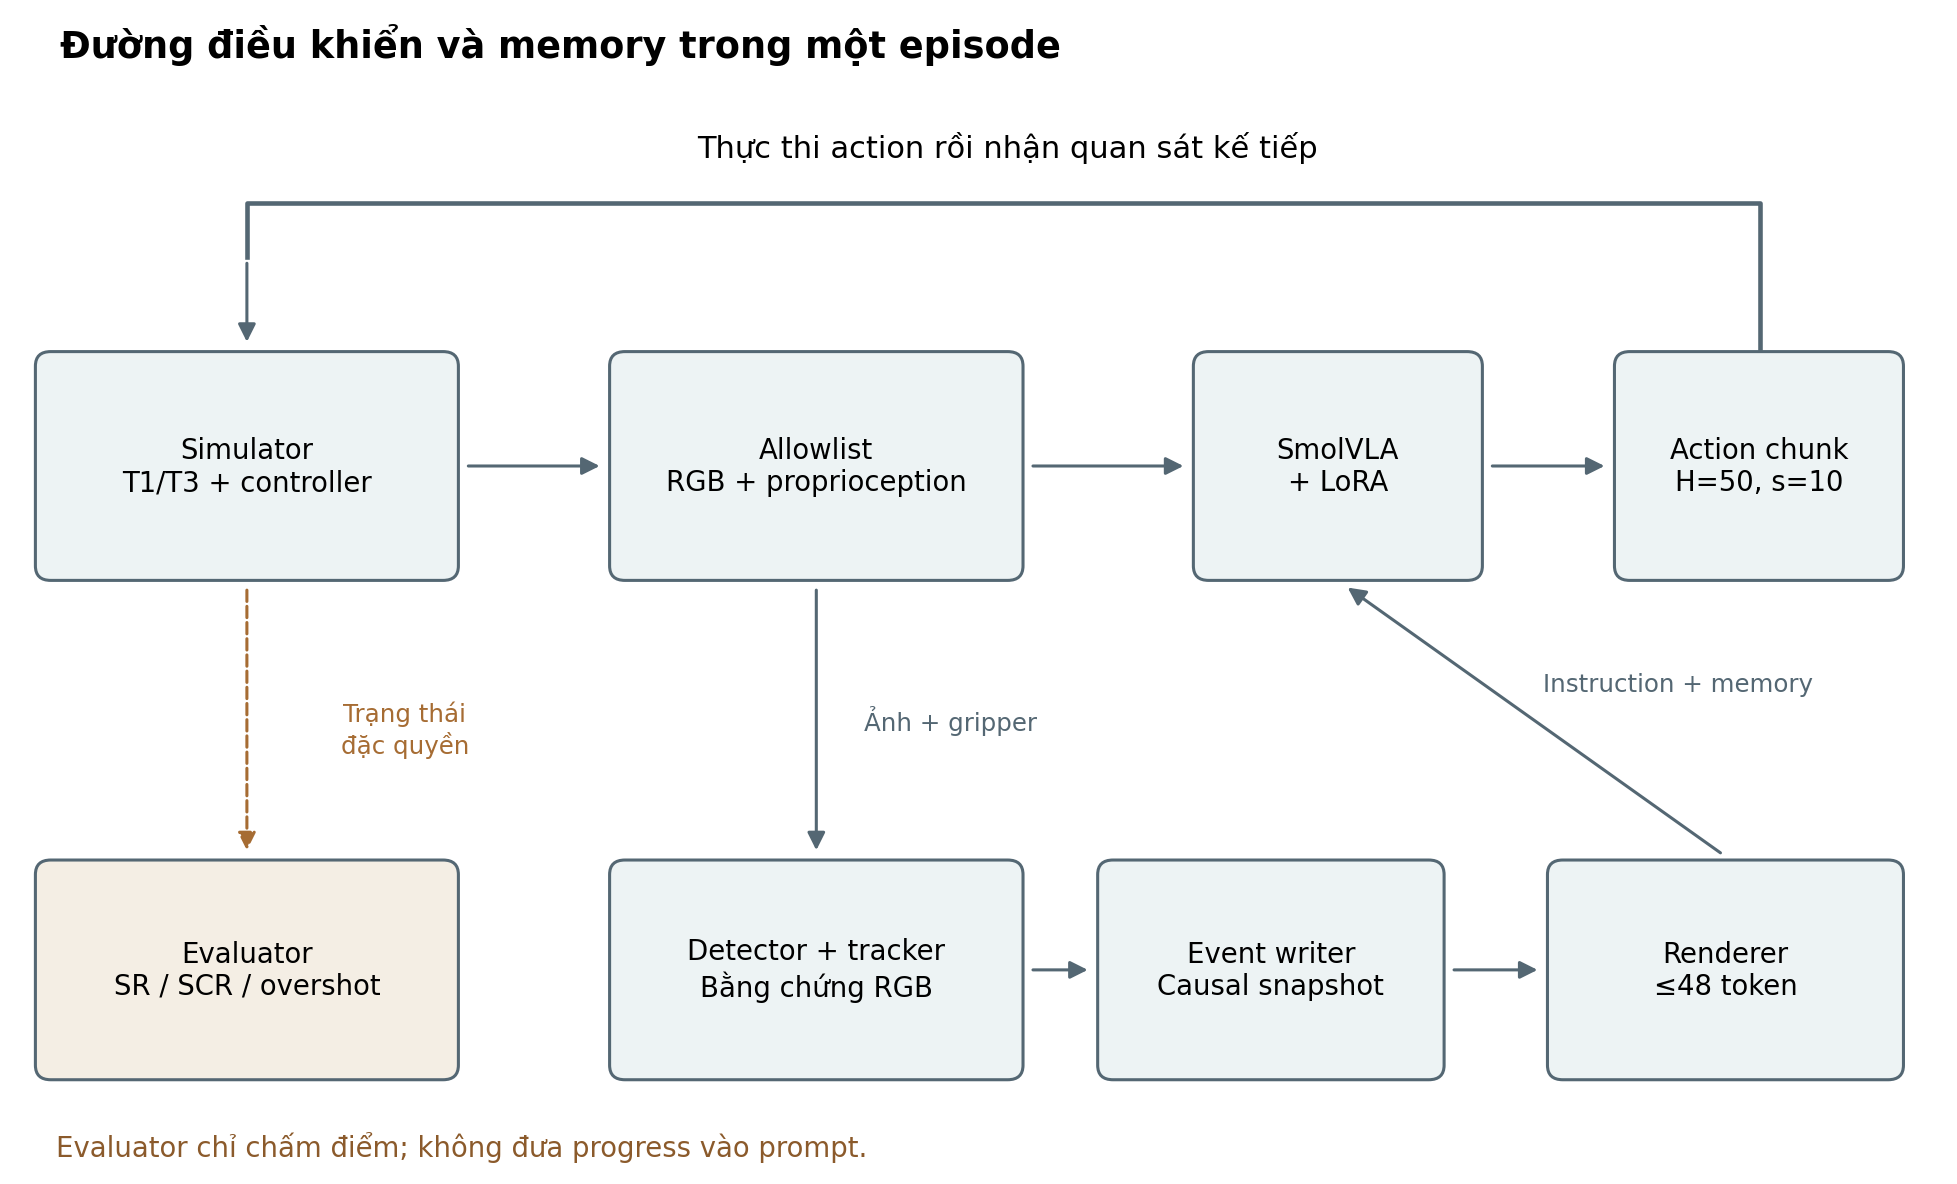
\includegraphics[width=\textwidth]{../figures/architecture.png}
\caption{Đường thông tin của phương pháp. Bộ nhớ được suy từ quan sát đã nhận, còn tiến độ do môi trường ghi nhận được dành cho đánh giá.}
\label{fig:architecture}
\end{figure}

Sự phân tách này đặc biệt quan trọng khi sinh mẫu huấn luyện từ quỹ đạo ghi sẵn. Một quỹ đạo đầy đủ có cả trạng thái sau thời điểm tạo mẫu và kết quả cuối lượt. Khi xây dựng ngữ cảnh cho một mẫu tại bước $t$, bộ ghi được cập nhật theo thứ tự thời gian và chỉ dựa trên tiền tố quan sát đến $t$. Thời điểm đủ bằng chứng cho từng sự kiện được lưu riêng để kiểm tra quy tắc này.

\section{Ước lượng quan hệ bát và đĩa gốc}

Giả định đo lường là trong bố trí của T1 và T3, một số thay đổi quan hệ bát và đĩa có thể được phát hiện từ chuyển động tương đối của các hộp giới hạn trong ảnh camera ngoài. Camera cổ tay cung cấp bằng chứng bổ trợ về khả năng quan sát. Đĩa gốc được neo bằng quan sát ở đầu lượt khi quan hệ bát trên đĩa đủ rõ và tay kẹp đã mở. Các quan sát sau phải ghép được với đĩa đã neo. Việc cố định tham chiếu theo thời gian giúp phép đo bám vào ngữ nghĩa “đặt về đĩa ban đầu”, kể cả khi bát xuất hiện gần đĩa khác.

Gọi $\mathbf b_t$ và $\mathbf q_t$ là tâm mép dưới hộp giới hạn của bát và đĩa ở bước $t$. Gọi $\mathbf b_0,\mathbf q_0$ là tọa độ tại lúc xác lập mốc tham chiếu, còn $w_b,h_b$ là chiều rộng và chiều cao hộp của bát tại thời điểm đó. Bộ theo dõi dùng ba đại lượng.

\begin{equation}
\begin{aligned}
d_t &= (\mathbf b_t-\mathbf q_t)-(\mathbf b_0-\mathbf q_0),\\
D_t &= \left\|d_t\oslash(w_b,h_b)\right\|_2,\qquad
L_t = -d_{t,y}/h_b .
\end{aligned}
\end{equation}

Ký hiệu $\oslash$ là phép chia theo từng thành phần. $D_t$ đo độ lệch khỏi quan hệ hình học lúc khởi đầu, đã chuẩn hóa theo kích thước biểu kiến của bát. $L_t$ đo thành phần dịch chuyển hướng lên trên mặt ảnh. Bộ theo dõi kết hợp $D_t$, $L_t$, tỷ lệ kích thước và độ ổn định theo thời gian. Độ mở đo từ hai khớp ngón kẹp bổ sung căn cứ cho việc xác nhận trạng thái nghỉ. Các ngưỡng trong cấu hình nghiên cứu được trình bày ở Bảng 3.1.

\begingroup\small\setlength{\tabcolsep}{4pt}\renewcommand{\arraystretch}{1.15}
\begin{longtable}{>{\raggedright\arraybackslash}p{\dimexpr 0.25\textwidth-2\tabcolsep\relax}>{\raggedright\arraybackslash}p{\dimexpr 0.35\textwidth-2\tabcolsep\relax}>{\raggedright\arraybackslash}p{\dimexpr 0.4\textwidth-2\tabcolsep\relax}}
\caption{Ngưỡng đo quan hệ giữa bát và đĩa gốc}\label{tab:generated2}\\
\toprule
\textbf{Đại lượng} & \textbf{Quy tắc trong cấu hình} & \textbf{Vai trò trong phép đo} \\
\midrule\endfirsthead
\toprule
\textbf{Đại lượng} & \textbf{Quy tắc trong cấu hình} & \textbf{Vai trò trong phép đo} \\
\midrule\endhead
\bottomrule\endfoot
Điểm phát hiện & $s_{\mathrm{det}}\ge 0{,}15$ & Lọc các hộp đề xuất theo điểm của bộ phát hiện \\
Tín hiệu nâng & $L_t\ge 0{,}40$ và nằm ngoài vùng gần đĩa gốc & Tạo ứng viên rời đĩa \\
Gần đĩa gốc & $D_t\le 0{,}30$. Tỷ lệ rộng từ $0{,}6$ đến $1{,}5$, cao từ $0{,}3$ đến $1{,}5$ & Tạo ứng viên quay về theo hình học ảnh \\
Ổn định & Độ dịch chuẩn hóa của tâm mép dưới $\le 0{,}15$ & Xác định bát ổn định so với quan sát gần nhất \\
Tay kẹp mở & Tổng trị tuyệt đối vị trí hai khớp ngón $\ge 0{,}055$ m & Bổ sung căn cứ để xác nhận bát đã được thả \\
Xác nhận theo thời gian & Ba quan sát phù hợp liên tiếp & Giảm xác nhận do nhiễu ở một khung ảnh \\
Ghép đĩa gốc & Độ dịch chuẩn hóa theo kích thước hộp đĩa neo $\le 0{,}45$ & Duy trì cùng đối tượng tham chiếu \\
Thu nhận mốc đĩa & Trong 20 bước đầu & Giới hạn thời điểm xác lập quan hệ ban đầu \\
\end{longtable}
\endgroup

Các phép đo trên mặt ảnh là chỉ dấu gián tiếp của quan hệ vật lý trong không gian ba chiều. Điểm phát hiện được dùng như tiêu chí chọn hộp, với ý nghĩa xác suất chưa được hiệu chuẩn. Trong trường hợp có nhiều hộp đề xuất, quan sát gần nhất có thể hỗ trợ ghép danh tính trong một khoảng thời gian giới hạn. Việc xác nhận ở bước hiện tại vẫn đòi hỏi quan sát phù hợp tại chính bước đó. Khi không định danh được bát hoặc không ghép được đĩa gốc, quan hệ ở bước hiện tại được ghi là chưa xác định. Các đặc điểm này giới hạn phạm vi áp dụng ở những cảnh có bố trí và góc nhìn tương tự.

\section{Ghi sự kiện và bất biến đếm chu kỳ}

Bộ ghi biểu diễn mỗi chu kỳ bằng một sự kiện rời đĩa và một sự kiện quay về theo đúng thứ tự. Quan hệ ban đầu được xác nhận khi bát ở gần đĩa gốc, ổn định và tay kẹp mở qua đủ số quan sát. Sau đó, tín hiệu nâng kéo dài tạo một sự kiện rời đĩa. Khi đã xác nhận sự kiện này, bộ ghi mới xét chuỗi quan sát bát về gần đĩa gốc, ổn định và tay kẹp mở để xác nhận sự kiện quay về. Mỗi lần xác nhận quay về kết thúc chu kỳ đang mở và tăng $\hat z_t$ một đơn vị.

Bộ ghi dùng trạng thái ứng viên để tích lũy bằng chứng. Khi bước quan sát bị bỏ qua hoặc không đủ căn cứ thị giác, ứng viên chưa xác nhận được xóa và cờ lịch sử chưa đầy đủ được đặt. Các sự kiện đã xác nhận được giữ. Nếu một chu kỳ đã mở trước khoảng trống, nó vẫn mở cho đến khi bộ ghi có bằng chứng phù hợp để xác nhận quay về. Số khoảng trống phản ánh mức độ gián đoạn của quan sát. Khi một khoảng trống có thể chứa sự kiện chưa được ghi nhận, từ $\hat z_t$ chưa thể khôi phục chính xác $z_t$. Nếu mọi lần quay về được xác nhận đều tương ứng đúng với các sự kiện thật phân biệt, $\hat z_t$ có thể được diễn giải như một cận dưới của số chu kỳ. Điều kiện đó cần được kiểm tra bằng dữ liệu có nhãn phù hợp.

\textbf{Mệnh đề 1 (bất biến đếm chu kỳ).} Trong một lượt thực thi với bộ ghi khởi tạo mới và các chuyển trạng thái hoàn tất theo quy tắc trên, mỗi lần tăng $\hat z_t$ đóng đúng một sự kiện rời đĩa đã xác nhận và chưa ghép cặp. Giữa hai lần tăng liên tiếp phải có một sự kiện rời đĩa mới.

\textbf{Chứng minh.} Gọi $J_t$ là số sự kiện rời đĩa đã xác nhận và $\chi_t\in\{0,1\}$ là cờ cho biết có một chu kỳ đang mở. Ở trạng thái khởi tạo, cả ba biến đều bằng không. Xét đẳng thức bất biến

\begin{equation}
J_t-\hat z_t=\chi_t.
\end{equation}

Chuyển xác nhận rời đĩa chỉ xảy ra khi $\chi_t=0$ trước chuyển và làm tăng $J_t$ một đơn vị đồng thời đặt $\chi_t=1$. Chuyển xác nhận quay về chỉ xảy ra khi $\chi_t=1$ trước chuyển và làm tăng $\hat z_t$ một đơn vị đồng thời đặt $\chi_t=0$. Các chuyển còn lại giữ nguyên $J_t$, $\hat z_t$ và $\chi_t$. Do đó đẳng thức đúng sau mọi chuyển theo quy nạp. Vì mỗi lần tăng $\hat z_t$ cần một chu kỳ đang mở và đóng chu kỳ đó, cùng một sự kiện rời đĩa chỉ ghép được với một lần tăng. Bất biến này ràng buộc cấu trúc của dãy sự kiện do bộ ghi tạo ra. Độ đúng của từng sự kiện so với thao tác vật lý còn phụ thuộc phép đo ở Mục 3.3.

\section{Tính không nhìn trước và biểu diễn văn bản}

Một sự kiện $e_j$ có thời điểm bắt đầu ước lượng $\tau_j$ và thời điểm đủ bằng chứng $\upsilon_j$. Chẳng hạn, nếu bộ ghi dùng ba khung ảnh liên tiếp từ bước 10 để xác nhận quay về, nó có thể gán $\tau_j=10$ và $\upsilon_j=12$. Sự kiện chỉ được sử dụng từ bước 12 trở đi. Tại bước truy vấn $q$, điều kiện thời gian và nguồn bằng chứng được biểu diễn bằng

\begin{equation}
\mathcal{E}_q =
\{e_j \mid \tau_j\le \upsilon_j\le q,\,
  \operatorname{source}(e_j)=\mathrm{RGB}\}.
\end{equation}

Nhãn nguồn $\mathrm{RGB}$ trong biểu thức chỉ các sự kiện do bộ theo dõi thị giác dự đoán và có căn cứ truy vết được. Bên cạnh thời điểm khả dụng, phép tạo văn bản kiểm tra sự nhất quán giữa danh tính bát, danh tính đĩa, số lần quay về và các sự kiện được tham chiếu. Dữ liệu lấy từ trạng thái đặc quyền của mô phỏng hoặc nhãn gán tay thuộc nguồn đánh giá. Phép tạo ngữ cảnh ở điều kiện F1 từ chối ảnh chụp bộ nhớ mang các nguồn này.

Chỉ dẫn gốc được giữ nguyên ở đầu ngữ cảnh. Phần bộ nhớ có thể mô tả số lần quay về đã xác nhận, chu kỳ đang mở hoặc lịch sử chưa đầy đủ. Ví dụ, ở bước truy vấn sau khi ghi nhận hai lần quay về trong T3, phần bổ sung có thể nêu rằng bát đã được quan sát quay lại đĩa gốc hai lần. Với lịch sử gián đoạn, cách diễn đạt phải thể hiện tính chưa đầy đủ của bằng chứng. Ngân sách là 48 token cho toàn bộ chỉ dẫn và phần bổ sung theo tokenizer của checkpoint, kể cả ký hiệu xuống dòng và token đặc biệt. Bộ dựng ngữ cảnh bỏ mệnh đề vượt ngân sách và ghi nhận lần bỏ đó. Chỉ dẫn tự vượt ngân sách làm dừng lượt chạy. Phạm vi của 48 token là đầu vào văn bản, còn số bằng chứng lưu trong suốt lượt có thể tăng theo độ dài quỹ đạo.

\textbf{Mệnh đề 2 (tính không nhìn trước của ngữ cảnh).} Cố định chỉ dẫn, cấu hình, định danh lượt và mọi nguồn ngẫu nhiên dùng để tạo bộ nhớ. Giả sử bộ ghi bắt đầu ở trạng thái mới, mỗi lần cập nhật chỉ nhận quan sát đến bước hiện tại và các hành động đã thực thi, đồng thời mỗi bằng chứng ảnh được ghép với đúng bước quan sát của nó. Giả sử phép tạo văn bản chỉ nhận trạng thái bộ nhớ hiện hành, kiểm tra $\upsilon_j\le q$ và từ chối các nguồn đặc quyền như trên. Khi đó, hai quỹ đạo có cùng tiền tố quan sát và hành động đã thực thi đến bước $q$ sẽ sinh cùng ngữ cảnh $c_q$, bất kể phần tiếp diễn của chúng.

\textbf{Chứng minh.} Cùng quan sát đầu và cùng cấu hình dẫn đến cùng trạng thái bộ nhớ ban đầu. Giả sử hai trạng thái bộ nhớ ở bước $t-1$ bằng nhau với $t\le q$. Hai tiền tố bằng nhau cho cùng $o_t$ và $a_{t-1}$, vì vậy quy tắc cập nhật $U$ cho cùng $m_t$. Quy nạp cho $m_q$ bằng nhau. Phép $R$ áp dụng cùng phép kiểm tra nguồn, thời điểm và ngân sách lên hai bản ghi giống nhau nên trả cùng $c_q$. Tính chất này có điều kiện trên việc cấp đúng bằng chứng quan sát theo thời gian. Nhãn nguồn và thời điểm được dùng để kiểm tra sự tuân thủ điều kiện đó. Độ đúng của nội dung sự kiện và mức độ chính sách sử dụng nội dung cần được xác định qua đánh giá thực nghiệm.

\section{Dữ liệu và thích ứng chính sách}

Dữ liệu thích ứng ghép các quỹ đạo mẫu LIBERO-10 với các quỹ đạo T1 và T3 từ bản phát hành của tác giả. Các quỹ đạo có cùng vector trạng thái khởi tạo được xếp vào cùng một nhóm trước khi chia tập. Định danh nhóm được tính từ vector đầy đủ ở biểu diễn float64 little-endian. Các nhóm từng dùng để phát triển bộ ghi được xếp vào tập huấn luyện. Cách chia này kiểm soát trường hợp cùng trạng thái khởi tạo xuất hiện dưới nhiều tên tác vụ hoặc mã quỹ đạo khác nhau. Lịch sử sử dụng tập kiểm tra trong phát triển và khả năng giao thoa với dữ liệu tiền huấn luyện vẫn ảnh hưởng đến diễn giải khả năng khái quát hóa.

Quy ước ảnh được xác định theo nguồn. Đối với hai camera, ảnh tinh chỉnh từ bản phát hành LIBERO-Mem được lật dọc một lần để trở về quy ước ảnh thô, còn ảnh kết xuất thô từ mô phỏng được giữ nguyên trước bộ tiền xử lý SmolVLA. Việc chuẩn hóa hướng ảnh giữ nguyên các phép biến đổi ảnh và quy tắc giải mã hành động của checkpoint. Adapter dùng trong Chương 4 được huấn luyện trên các quỹ đạo từ bản phát hành. Bộ dữ liệu phát lại theo cấu hình mô phỏng cục bộ còn cần hoàn tất kiểm chứng trước khi dùng để đánh giá một adapter mới.

Thích ứng được thực hiện bằng LoRA tại các phép chiếu query và value của attention trong mô-đun sinh hành động. Các trọng số nền được giữ cố định, cùng với bộ chuẩn hóa trạng thái và phép giải chuẩn hành động của checkpoint. Mỗi lô tối ưu hóa gồm dữ liệu thao tác cơ sở và dữ liệu T1/T3. Bộ lấy mẫu cân bằng theo tác vụ trong từng miền và chọn quỹ đạo trước khi lấy khung ảnh, nhằm hạn chế ảnh hưởng của chênh lệch độ dài giữa các quỹ đạo. Trộn dữ liệu cơ sở tạo điều kiện khảo sát khả năng duy trì kỹ năng sau thích ứng. Kết luận về khả năng duy trì đòi hỏi đánh giá chính adapter trên các tác vụ cơ sở dưới cùng quy trình.

\section{Thiết kế đối chứng}

Các đối chứng được xác định theo câu hỏi mà từng phép so sánh có thể trả lời. B0 là mốc tham chiếu với trọng số gốc. Để đo thay đổi do thích ứng, F0 cần dùng cùng tập quỹ đạo, cách chia, cấu hình, ngân sách huấn luyện và quy tắc chọn checkpoint như F1, với ngữ cảnh huấn luyện và suy luận chỉ chứa chỉ dẫn. F1 bổ sung biểu diễn sự kiện trong cả thích ứng lẫn suy luận. F1-off giữ nguyên trọng số F1 và bỏ phần sự kiện ở thời điểm suy luận.

\begingroup\small\setlength{\tabcolsep}{4pt}\renewcommand{\arraystretch}{1.15}
\begin{longtable}{>{\raggedright\arraybackslash}p{\dimexpr 0.29\textwidth-2\tabcolsep\relax}>{\raggedright\arraybackslash}p{\dimexpr 0.1775\textwidth-2\tabcolsep\relax}>{\raggedright\arraybackslash}p{\dimexpr 0.1775\textwidth-2\tabcolsep\relax}>{\raggedright\arraybackslash}p{\dimexpr 0.1775\textwidth-2\tabcolsep\relax}>{\raggedright\arraybackslash}p{\dimexpr 0.1775\textwidth-2\tabcolsep\relax}}
\caption{Các điều kiện đối chứng và mục đích đánh giá}\label{tab:generated3}\\
\toprule
\textbf{Điều kiện} & \textbf{Trọng số} & \textbf{Ngữ cảnh suy luận} & \textbf{Mục đích đánh giá} & \textbf{Bằng chứng hiện có} \\
\midrule\endfirsthead
\toprule
\textbf{Điều kiện} & \textbf{Trọng số} & \textbf{Ngữ cảnh suy luận} & \textbf{Mục đích đánh giá} & \textbf{Bằng chứng hiện có} \\
\midrule\endhead
\bottomrule\endfoot
B0 & Checkpoint gốc & Chỉ dẫn & Mốc tham chiếu trước thích ứng & 20 lượt T1/T3 \\
F0 & Adapter huấn luyện đối sánh & Chỉ dẫn & Đối chứng cho thay đổi do thích ứng & Chưa có lượt chạy đối sánh \\
F1 & Adapter học với bộ nhớ & Chỉ dẫn và sự kiện & Đánh giá phương pháp đề xuất & 20 lượt T1/T3 \\
F1-off & Cùng adapter F1 & Chỉ dẫn & Đo độ nhạy với việc bỏ phần sự kiện & Chưa có lượt chạy vòng kín \\
\end{longtable}
\endgroup

So sánh hiện có B0 với F1 đo chênh lệch khi thay đồng thời trọng số thích ứng và nguồn ngữ cảnh. So sánh F0 với F1 ở cùng ngân sách sẽ thu hẹp câu hỏi về giá trị của việc bổ sung nhánh bộ nhớ. Để nghiên cứu riêng giá trị của thông tin lịch sử, một đối chứng bổ sung có thể cung cấp tóm tắt quan sát hiện tại bằng cùng bộ phát hiện. Một đối chứng khác có thể giữ ngân sách token tương đương và dùng phần bổ sung không mang tín hiệu tiến độ. F1-off có ý nghĩa chẩn đoán độ nhạy của cùng trọng số với ngữ cảnh. Do phần bộ nhớ chưa được bỏ ngẫu nhiên khi huấn luyện F1, việc bỏ phần này lúc suy luận có thể đưa ngữ cảnh ra ngoài phân phối huấn luyện. Các đối chứng này xác định hướng kiểm tra giả thuyết mà các lượt B0 và F1 hiện có chưa phân giải được.

\section{Quy trình đánh giá và độ đo}

Hai cấu hình đã chạy dùng robot Panda với bộ điều khiển OSC\_POSE ở 20 Hz, hai ảnh kích thước $256\times256$ và cùng danh sách trạng thái khởi tạo đã khóa. Mỗi lượt có 20 bước làm nóng theo quy trình trước khi tính các bước của chính sách. SmolVLA dự đoán đoạn $H=50$ hành động và thực thi $s=10$ hành động trước khi truy vấn lại. Bộ ghi cập nhật sau từng hành động, vì sự kiện có thể được xác nhận giữa hai lần truy vấn.

Mỗi lượt có giới hạn 1.000 hành động do chính sách sinh và dừng sớm khi bộ chấm ghi nhận vượt mục tiêu. Một trạng thái hoàn tất xuất hiện giữa lượt vẫn phải được duy trì theo quy tắc chấm ở thời điểm kết thúc. Quy tắc này giữ yêu cầu kết thúc đúng tiến độ, vốn là phần quan trọng của tác vụ lặp. Bộ chấm đọc tiến độ và vị từ từ bản mã đánh giá LIBERO-Mem đã cố định phiên bản. Kết quả được diễn giải trong phạm vi quy trình mô phỏng cục bộ đã khai báo.

Với lượt $i$, gọi $K_i$ là số mốc được bộ chấm xác nhận, $K_i^\star$ là số mốc cần đạt, $P_i$ là vị từ đích tại thời điểm kết thúc và $O_i$ là cờ vượt mục tiêu. Gọi $M$ là số lượt hoàn tất đánh giá trong nhóm đang xét. Các độ đo gồm chỉ báo thành công $S_i$, tỷ lệ hoàn thành mốc $\mathrm{SCR}_i$ và tỷ lệ thành công thực nghiệm $\widehat{\mathrm{SR}}$.

\begin{equation}
\begin{aligned}
S_i &= \mathbf{1}[K_i=K_i^\star\land P_i\land\neg O_i],\\
\mathrm{SCR}_i &= K_i/K_i^\star,\qquad
\widehat{\mathrm{SR}} = \frac{1}{M}\sum_{i=1}^{M}S_i.
\end{aligned}
\end{equation}

$\mathrm{SCR}_i$ phản ánh tiến độ từng phần. $S_i$ còn yêu cầu trạng thái đích hợp lệ ở điểm cuối và dừng trong giới hạn số lần lặp. Hai tác vụ có cùng số lượt trong mỗi cấu hình đã chạy, nên trung bình tỷ lệ thành công theo tác vụ bằng tỷ lệ tính trên tất cả các lượt của cấu hình. Trạng thái khởi tạo được ghép giữa B0 và F1, đồng thời được dùng lại giữa T1 và T3. Cách ghép này cho phép đối chiếu từng trường hợp nhưng tạo phụ thuộc giữa các quan sát chung trạng thái. Việc phân tích vì vậy cần giữ thông tin nhóm trạng thái, số seed và điều kiện dừng của từng lượt.


\chapter{Thực nghiệm và thảo luận}

\section{Phạm vi suy luận thực nghiệm}

Để hỗ trợ điều khiển, một biểu diễn tiến độ cần thỏa mãn ba điều kiện: có thể suy ra từ quan sát khả dụng, đến được chính sách đúng lúc và chứa thông tin mà chính sách có thể sử dụng để chọn hành động. Khóa luận xem xét ba loại bằng chứng: sự phù hợp của sự kiện với mốc tiến độ trong các quỹ đạo thao tác mẫu, độ nhạy của sai số dự đoán hành động đối với đầu vào bộ nhớ, và kết quả điều khiển vòng kín. Đối chiếu ba phép đo giúp xác định mắt xích nào đã có bằng chứng và mắt xích nào cần một phép can thiệp riêng.

Nguồn phân tích chính gồm phép phát lại sáu quỹ đạo thao tác mẫu ngày 26/10/2026, nhật ký xác thực của mô hình F1 và 40 quỹ đạo điều khiển hoàn tất trong đợt đánh giá ngày 09/11/2026. Với đợt đánh giá vòng kín, số liệu được tính lại từ từng bản tóm tắt quỹ đạo, sau khi đối chiếu tổng kiểm, trạng thái hoàn tất, tác vụ, trạng thái khởi tạo và hạt giống. Danh mục dữ liệu, phiên bản và tổng kiểm được lưu cùng bản ghi thực nghiệm ngày 12/11/2026 \cite{artifact2026}.

Đối chứng của phân tích vòng kín là B0 trên chính T1/T3. Kết quả V1 trong phụ lục chỉ cung cấp bối cảnh về chính sách gốc trên các tác vụ khác và với nhịp truy vấn khác. \cite{artifact2026}

\section{Mức phù hợp giữa sự kiện thị giác và mốc tiến độ}

Để khảo sát RQ2, bộ ghi sự kiện từ RGB được áp dụng trên sáu quỹ đạo thao tác mẫu T1/T3, gồm 1.276 khung hình và ba trạng thái khởi tạo. Với mỗi trạng thái đều có quỹ đạo của cả T1 lẫn T3. Hai quỹ đạo được dùng để phát triển phương pháp và các quỹ đạo bổ sung cũng đã được quan sát trước khi tổng hợp. Phép đo này vì vậy có phạm vi chẩn đoán trên những quỹ đạo đã biết. Nhãn tham chiếu mô tả thời điểm tiến độ tích lũy đạt mốc, nên phù hợp để đối chiếu sự kiện hoàn thành chu kỳ, còn thời điểm tiếp xúc hoặc nhả vật cần một loại nhãn khác.

Mỗi sự kiện đặt lại do bộ ghi xác nhận được ghép với nhiều nhất một mốc tham chiếu, trong dung sai 20 khung hình. Tất cả 12 sự kiện xác nhận đều ghép được với 12 mốc. Độ trễ xác nhận có trung vị 9 khung hình, trung bình xấp xỉ 9,92 khung hình và nằm trong khoảng 6–20 khung hình. Kết quả cho thấy có thể trích xuất một biến tiến độ hữu ích để mô tả những quỹ đạo đã xem từ bằng chứng thị giác. Độ trễ quan sát được cho thấy giữa thời điểm tiến độ thay đổi và thời điểm chính sách có thể nhận bằng chứng về thay đổi đó tồn tại một khoảng chờ cần tính đến.

\begingroup\small\setlength{\tabcolsep}{4pt}\renewcommand{\arraystretch}{1.15}
\begin{longtable}{>{\raggedright\arraybackslash}p{\dimexpr 0.25\textwidth-2\tabcolsep\relax}>{\raggedright\arraybackslash}p{\dimexpr 0.35\textwidth-2\tabcolsep\relax}>{\raggedright\arraybackslash}p{\dimexpr 0.4\textwidth-2\tabcolsep\relax}}
\caption{Đối chiếu sự kiện thị giác với mốc tiến độ trên các quỹ đạo mẫu}\label{tab:generated4}\\
\toprule
\textbf{Đại lượng khảo sát} & \textbf{Kết quả quan sát} & \textbf{Phạm vi diễn giải} \\
\midrule\endfirsthead
\toprule
\textbf{Đại lượng khảo sát} & \textbf{Kết quả quan sát} & \textbf{Phạm vi diễn giải} \\
\midrule\endhead
\bottomrule\endfoot
Quỹ đạo mẫu / trạng thái / khung hình & 6 / 3 / 1.276 & Các quỹ đạo hoàn thành tác vụ đã được quan sát \\
Mốc tham chiếu / sự kiện xác nhận / cặp ghép & 12 / 12 / 12 & Ghép một-một trong dung sai ±20 khung hình \\
Sự kiện dư / mốc bị bỏ sót & 0 / 0 & Tính trên sáu quỹ đạo mẫu \\
Độ trễ xác nhận & Trung vị 9, khoảng 6–20 khung hình & So với mốc tham chiếu \\
Phát hiện bát có IoU $\geq0{,}5$ & 1.169/1.172 (99,74\%) & Mẫu số chỉ gồm phát hiện đã được bộ theo dõi chấp nhận \\
Có định vị vật / có văn bản bộ nhớ & 1.172/1.276 / 1.258/1.276 khung hình & Tỷ lệ có đầu ra ở từng khâu \\
Lời nhắc dài nhất & 31 trên giới hạn 48 token & Đo bằng bộ tách token đã chọn \\
Độ trễ xử lý RGB & Khoảng 999–1.058 ms/khung hình & Độ trễ tính toán ở lần đo riêng \\
\end{longtable}
\endgroup

Tỷ lệ khớp hộp giới hạn đo chất lượng định vị có điều kiện trên các phát hiện được chấp nhận. Tỷ lệ này bỏ qua các khung mà đối tượng bị bỏ sót hoặc bị từ chối. Tương tự, việc tạo được văn bản chỉ chứng tỏ biểu diễn có đầu ra tại khung hình đó. Muốn ước lượng mức phù hợp của nội dung bộ nhớ trên phân phối điều khiển, cần cả quỹ đạo thành công lẫn thất bại và nhãn độc lập cho những tình huống như nhấc hụt, đặt lệch đĩa hoặc che khuất kéo dài.

Phụ lục ghi nguồn dữ liệu, phương pháp đối chiếu và các phép kiểm tính nhất quán của quá trình tạo bản ghi. \cite{artifact2026}

\section{Điều kiện đối chiếu trong mô phỏng}

Việc so sánh vòng kín giữa các chính sách đòi hỏi giữ ổn định động lực học, điều kiện quan sát và tiêu chí chấm điểm. Mức độ quy kết còn phụ thuộc vào những thành phần được thay đổi trong phép đối chứng. Hai lần chạy B0/F1 có cùng tổng kiểm của mô hình gốc, cấu hình đánh giá và danh sách trạng thái. Bản ghi nguồn của hai lần chạy khác nhau ở ba tập lệnh khởi chạy hoặc chẩn đoán. Các điểm khớp giúp thu hẹp diễn giải về biến gây nhiễu, còn khác biệt nguồn đặt giới hạn cho phát biểu về độ tương đương của hai lần chạy. Phụ lục mô tả quy trình đối chiếu bản ghi \cite{artifact2026}.

\begingroup\small\setlength{\tabcolsep}{4pt}\renewcommand{\arraystretch}{1.15}
\begin{longtable}{>{\raggedright\arraybackslash}p{\dimexpr 0.31\textwidth-2\tabcolsep\relax}>{\raggedright\arraybackslash}p{\dimexpr 0.69\textwidth-2\tabcolsep\relax}}
\caption{Các điều kiện đối chiếu trong thực nghiệm vòng kín}\label{tab:generated5}\\
\toprule
\textbf{Điều kiện} & \textbf{Giá trị dùng trong thực nghiệm} \\
\midrule\endfirsthead
\toprule
\textbf{Điều kiện} & \textbf{Giá trị dùng trong thực nghiệm} \\
\midrule\endhead
\bottomrule\endfoot
Mô hình gốc & SmolVLA cho LIBERO, cùng phiên bản ở B0 và F1 \\
Nguồn tác vụ và bộ chấm & LIBERO-Mem tại phiên bản đã khóa \\
Mô phỏng & Franka Panda trong robosuite 1.4.0, cùng thiết lập động lực học \\
Đầu vào chính sách & Hai camera 256×256, trạng thái 8 chiều, tiền xử lý theo checkpoint gốc \\
Điều khiển & OSC\_POSE ở 20 Hz trong mô phỏng, dự đoán $H=50$, thực thi $s=10$ \\
Khởi tạo và điểm cuối & Trạng thái từ danh sách đã khóa, 20 bước làm ấm, tối đa 1.000 hành động chính sách, dừng sớm khi vượt số chu kỳ \\
\end{longtable}
\endgroup

Huấn luyện sử dụng hai GPU Tesla T4. Phép đánh giá dùng NVIDIA GeForce RTX 4060 Laptop, với mô phỏng chạy trong WSL và suy luận chính sách trên Windows. Những điều kiện này xác định môi trường áp dụng của kết quả. Chu kỳ danh định 20 Hz của bộ điều khiển tương ứng 50 ms mỗi bước mô phỏng. Riêng thời gian xử lý một khung hình RGB trong phép đo chẩn đoán đã xấp xỉ một giây. Thời gian phát lại máy trạng thái từ dữ liệu đã lưu khoảng 1–2 ms mỗi khung hình phản ánh chi phí của một thành phần khác, sau khi đã có kết quả nhận dạng vật. Khi mô phỏng tạm dừng để chờ suy luận, tiến độ mô phỏng và thời gian thực trôi qua là hai đại lượng khác nhau. Một kết luận về khả năng vận hành thời gian thực cần đo trọn chu trình trên cấu hình đã xác định.

\section{Mẫu nghiên cứu và điều kiện thích ứng}

Tập dữ liệu huấn luyện kết hợp quỹ đạo thao tác cơ sở LIBERO-10 với quỹ đạo T1/T3 từ nguồn LIBERO-Mem của tác giả. Bảng dưới ghi số quỹ đạo trong danh mục dữ liệu được dùng để huấn luyện F1. Các quỹ đạo có cùng mã băm trạng thái khởi tạo được phân vào cùng một tập. Trong tập kiểm tra T1/T3, 20 tổ hợp tác vụ và trạng thái của mỗi điều kiện tương ứng 10 nhóm trạng thái dùng chung giữa hai tác vụ. Tập này đã được sử dụng trong quá trình phát triển. Vì vậy, số liệu vòng kín phù hợp cho phân tích thăm dò và hình thành giả thuyết kiểm chứng.

\begingroup\small\setlength{\tabcolsep}{4pt}\renewcommand{\arraystretch}{1.15}
\begin{longtable}{>{\raggedright\arraybackslash}p{\dimexpr 0.29\textwidth-2\tabcolsep\relax}>{\raggedright\arraybackslash}p{\dimexpr 0.1775\textwidth-2\tabcolsep\relax}>{\raggedright\arraybackslash}p{\dimexpr 0.1775\textwidth-2\tabcolsep\relax}>{\raggedright\arraybackslash}p{\dimexpr 0.1775\textwidth-2\tabcolsep\relax}>{\raggedright\arraybackslash}p{\dimexpr 0.1775\textwidth-2\tabcolsep\relax}}
\caption{Phân hoạch quỹ đạo theo nhóm tác vụ}\label{tab:generated6}\\
\toprule
\textbf{Nhóm dữ liệu} & \textbf{Huấn luyện} & \textbf{Xác thực} & \textbf{Kiểm tra} & \textbf{Tổng} \\
\midrule\endfirsthead
\toprule
\textbf{Nhóm dữ liệu} & \textbf{Huấn luyện} & \textbf{Xác thực} & \textbf{Kiểm tra} & \textbf{Tổng} \\
\midrule\endhead
\bottomrule\endfoot
Thao tác cơ sở LIBERO-10 & 400 & 50 & 50 & 500 \\
Mem T1 & 80 & 10 & 10 & 100 \\
Mem T3 & 78 & 10 & 10 & 98 \\
Tổng & 558 & 70 & 70 & 698 \\
\end{longtable}
\endgroup

Lấy mẫu hỗn hợp nhằm đặt ra bài toán duy trì kỹ năng cơ sở (RQ3) trong cùng quá trình thích ứng với tác vụ phụ thuộc lịch sử. Trong mỗi lô cập nhật, số mẫu của hai miền được phân bổ theo tỷ lệ đã chọn. Trong từng miền, tác vụ được chọn luân phiên, sau đó lấy mẫu đều theo quỹ đạo rồi chọn khung hình. Cách này làm giảm ảnh hưởng của độ dài quỹ đạo lên xác suất được chọn. Tỷ lệ lấy mẫu 50/50 là một điều kiện huấn luyện đã quan sát, nên giá trị của việc trộn dữ liệu và lựa chọn tỷ lệ vẫn cần đối chứng riêng.

\begingroup\small\setlength{\tabcolsep}{4pt}\renewcommand{\arraystretch}{1.15}
\begin{longtable}{>{\raggedright\arraybackslash}p{\dimexpr 0.18\textwidth-2\tabcolsep\relax}>{\raggedright\arraybackslash}p{\dimexpr 0.23\textwidth-2\tabcolsep\relax}>{\raggedright\arraybackslash}p{\dimexpr 0.26\textwidth-2\tabcolsep\relax}>{\raggedright\arraybackslash}p{\dimexpr 0.33\textwidth-2\tabcolsep\relax}}
\caption{Cấu hình thích ứng của F1 và phạm vi suy luận}\label{tab:generated7}\\
\toprule
\textbf{Hạng mục} & \textbf{Cấu hình đã sử dụng} & \textbf{Vai trò nghiên cứu} & \textbf{Giới hạn suy luận} \\
\midrule\endfirsthead
\toprule
\textbf{Hạng mục} & \textbf{Cấu hình đã sử dụng} & \textbf{Vai trò nghiên cứu} & \textbf{Giới hạn suy luận} \\
\midrule\endhead
\bottomrule\endfoot
Vị trí thích ứng & LoRA tại phép chiếu query/value của khối sinh hành động, hạng 16, 645.120 tham số được cập nhật & Giữ mô hình nền cố định khi thích ứng & Chỉ khảo sát một vị trí và một hạng \\
Tối ưu hóa & AdamW, tốc độ học ban đầu $2\times10^{-5}$, làm ấm 100 bước, 3.000 bước cập nhật, chặn chuẩn gradient 1,0 & Cố định ngân sách của F1 & Chưa có khảo sát siêu tham số \\
Lấy mẫu hỗn hợp & Lô hiệu dụng 32, tỷ lệ dữ liệu cơ sở 0,5, hạt giống 42 & Đặt kỹ năng cơ sở và thích ứng vào cùng bài toán huấn luyện & Mức độ duy trì cần đo bằng điều khiển vòng kín \\
Bộ nhớ khi huấn luyện & Tỷ lệ bỏ bộ nhớ bằng 0, xác thực và lưu mô hình mỗi 500 bước & Xác định phân phối đầu vào của F1 & Bỏ bộ nhớ khi suy luận có thể thay đổi phân phối \\
Mô hình được đánh giá & Trọng số LoRA lưu riêng, dùng checkpoint ở bước 3.000 & Cố định phiên bản dùng cho các phép đo & Chưa chọn checkpoint theo tỷ lệ thành công vòng kín \\
\end{longtable}
\endgroup

Tổng kiểm của danh mục dữ liệu khớp với bản ghi huấn luyện, và bốn tệp được liệt kê trong bản xuất F1 có tổng kiểm khớp bản kê. Phép đối chiếu giới hạn ở các tệp đã nêu. Dữ liệu Mem của F1 dùng các quỹ đạo do tác giả công bố, với ảnh được đưa về quy ước gốc trước khi áp dụng tiền xử lý của chính sách. Một đợt tái tạo dữ liệu tại chỗ ghi nhận 73 trên 78 quỹ đạo phát lại T3 đạt điều kiện thành công của đợt phát lại. Các quỹ đạo đó là một nhánh nghiên cứu riêng. Chuỗi xác thực dữ liệu dẫn xuất, lập chỉ mục và huấn luyện trên phiên bản derived-v1 chưa hoàn tất, nên phân tích F1 căn cứ vào tập dữ liệu của tác giả \cite{artifact2026}.

\section{Độ nhạy ngoại tuyến đối với thông tin bộ nhớ}

Tại bước 3.000, trên 4.299 mẫu khung hình của tập xác thực Mem, hàm mất mát flow matching của cùng F1 là 0,23023575 khi có bộ nhớ và 0,33553660 khi bỏ bộ nhớ. Trên 13.525 mẫu khung hình của tập xác thực cơ sở, hai chế độ đều cho giá trị 0,42984212. Các khung hình được lấy từ quỹ đạo và có thể phụ thuộc theo thời gian. Phép so sánh giữ cố định trọng số F1 và thay đổi cách cung cấp bộ nhớ ở đầu vào.

\begin{figure}[htbp]
\centering
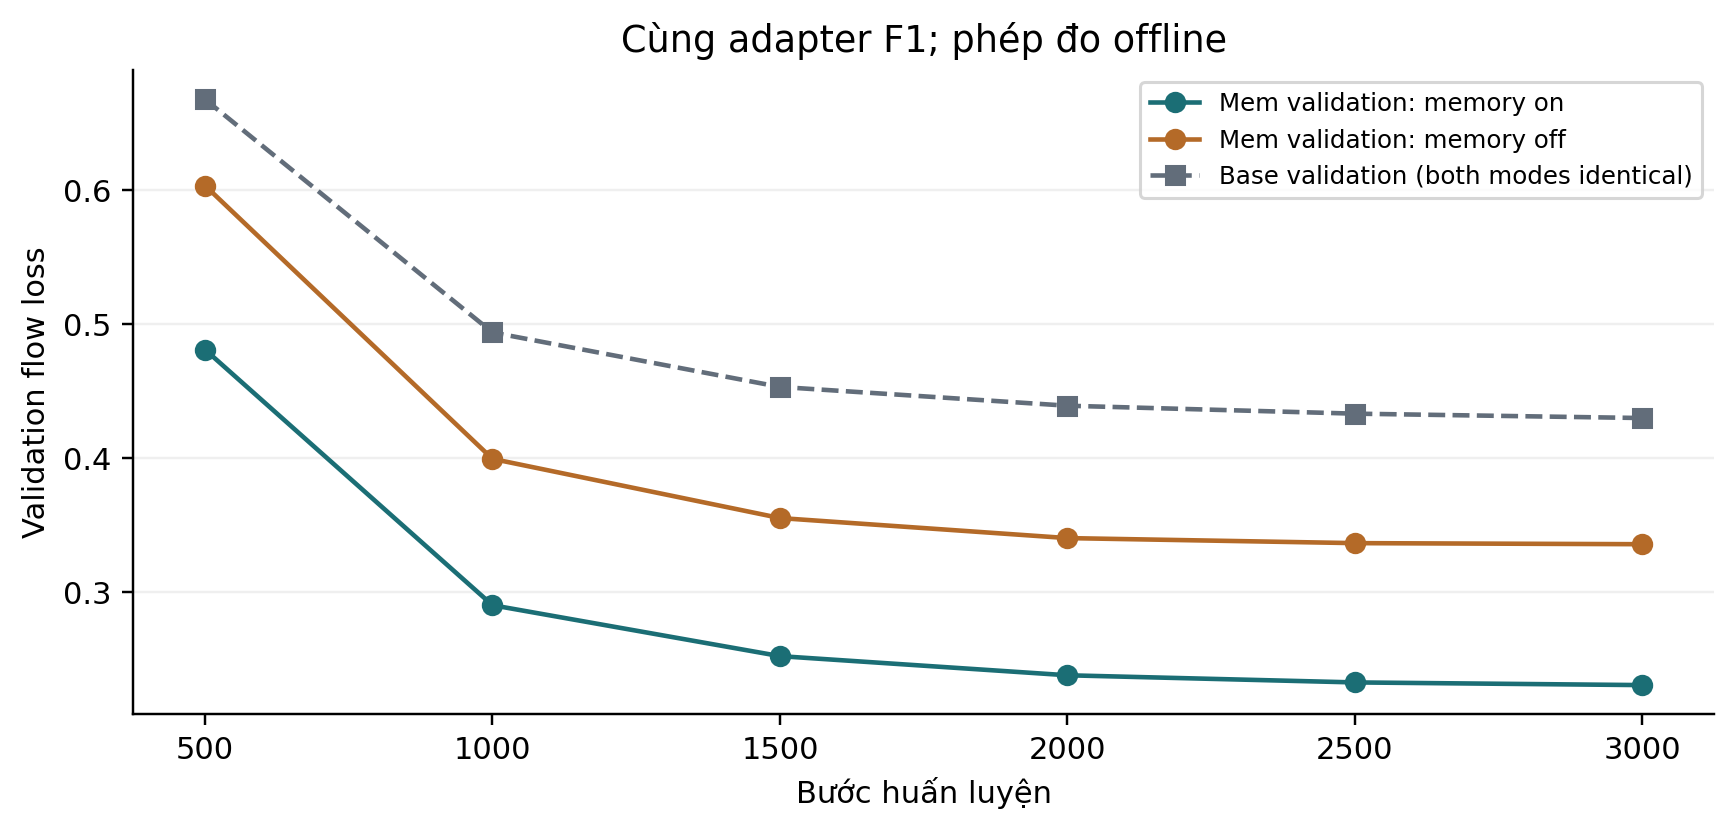
\includegraphics[width=\textwidth]{../figures/validation_loss.png}
\caption{Hàm mất mát flow matching trên tập xác thực theo số bước huấn luyện. Hai chế độ có và bỏ bộ nhớ được đo trên cùng checkpoint ở mỗi bước.}
\label{fig:validation_loss}
\end{figure}

Chênh lệch trên tập Mem là bằng chứng rằng cách cung cấp đầu vào bộ nhớ có liên hệ với chất lượng dự đoán hành động trên phân phối xác thực. Do F1 được huấn luyện với tỷ lệ bỏ bộ nhớ bằng 0, phép bỏ bộ nhớ có thể đồng thời loại thông tin tiến độ và đưa đầu vào ra ngoài phân phối huấn luyện. Để tách hai cách giải thích này, một phép thử có kiểm soát cần duy trì định dạng và dung lượng lời nhắc, đồng thời thay đổi có chủ đích thông tin lịch sử mà nó chứa. Mặt khác, một chính sách có sai số dự đoán nhỏ trên các quỹ đạo thao tác mẫu vẫn có thể thực thi kém khi các hành động của chính nó làm thay đổi phân phối quan sát.

Về khả năng duy trì kỹ năng trong RQ3, hai giá trị hàm mất mát bằng nhau trên tập cơ sở chỉ phản ánh tính ổn định giữa hai chế độ đầu vào của F1 trong phép đo này. Chẳng hạn, các mẫu cơ sở có thể có cùng đầu vào ở hai chế độ nếu chúng đều không mang hậu tố bộ nhớ. Để ước lượng mức duy trì kỹ năng, phép so sánh cần đặt chính F1 và B0 vào cùng các tác vụ cơ sở, với tiêu chí thành công và ngân sách điều khiển giống nhau.

\section{Kết quả điều khiển vòng kín}

RQ1 đặt vấn đề liệu lịch sử có giúp chính sách hoàn thành tác vụ khi đã kiểm soát thích ứng mô hình. Dữ liệu hiện có đối chiếu B0, tức checkpoint gốc, với F1, tức cấu hình có cả thích ứng và bộ nhớ quan sát trực tuyến. Đây là phép so sánh sơ bộ hai cấu hình nghiên cứu. Mỗi điều kiện dùng cùng 20 tổ hợp tác vụ và trạng thái, với hạt giống chính sách 42. Kết quả áp dụng cho giao thức T1/T3 của khóa luận, với nhãn \path{CUSTOM_V2_LIBERO_MEM} và \path{NON-COMPARABLE_OFFICIAL_PAPER}.

\begingroup\small\setlength{\tabcolsep}{4pt}\renewcommand{\arraystretch}{1.15}
\begin{longtable}{>{\raggedright\arraybackslash}p{\dimexpr 0.12\textwidth-2\tabcolsep\relax}>{\raggedright\arraybackslash}p{\dimexpr 0.14\textwidth-2\tabcolsep\relax}>{\raggedright\arraybackslash}p{\dimexpr 0.2\textwidth-2\tabcolsep\relax}>{\raggedright\arraybackslash}p{\dimexpr 0.12\textwidth-2\tabcolsep\relax}>{\raggedright\arraybackslash}p{\dimexpr 0.19\textwidth-2\tabcolsep\relax}>{\raggedright\arraybackslash}p{\dimexpr 0.23\textwidth-2\tabcolsep\relax}}
\caption{Kết quả điều khiển vòng kín theo tác vụ và điều kiện}\label{tab:generated8}\\
\toprule
\textbf{Nhiệm vụ} & \textbf{Điều kiện} & \textbf{Thành công / số lượt} & \textbf{SR} & \textbf{SCR trung bình} & \textbf{Vượt số chu kỳ / số lượt} \\
\midrule\endfirsthead
\toprule
\textbf{Nhiệm vụ} & \textbf{Điều kiện} & \textbf{Thành công / số lượt} & \textbf{SR} & \textbf{SCR trung bình} & \textbf{Vượt số chu kỳ / số lượt} \\
\midrule\endhead
\bottomrule\endfoot
T1 & B0 & 0/10 & 0\% & 0,1000 & 1/10 \\
T1 & F1 & 0/10 & 0\% & 0,1000 & 1/10 \\
T3 & B0 & 0/10 & 0\% & 0,0000 & 0/10 \\
T3 & F1 & 1/10 & 10\% & 0,1667 & 0/10 \\
Hai tác vụ & B0 & 0/20 & 0\% & 0,0500 & 1/20 \\
Hai tác vụ & F1 & 1/20 & 5\% & 0,1333 & 1/20 \\
\end{longtable}
\endgroup

\begin{figure}[htbp]
\centering
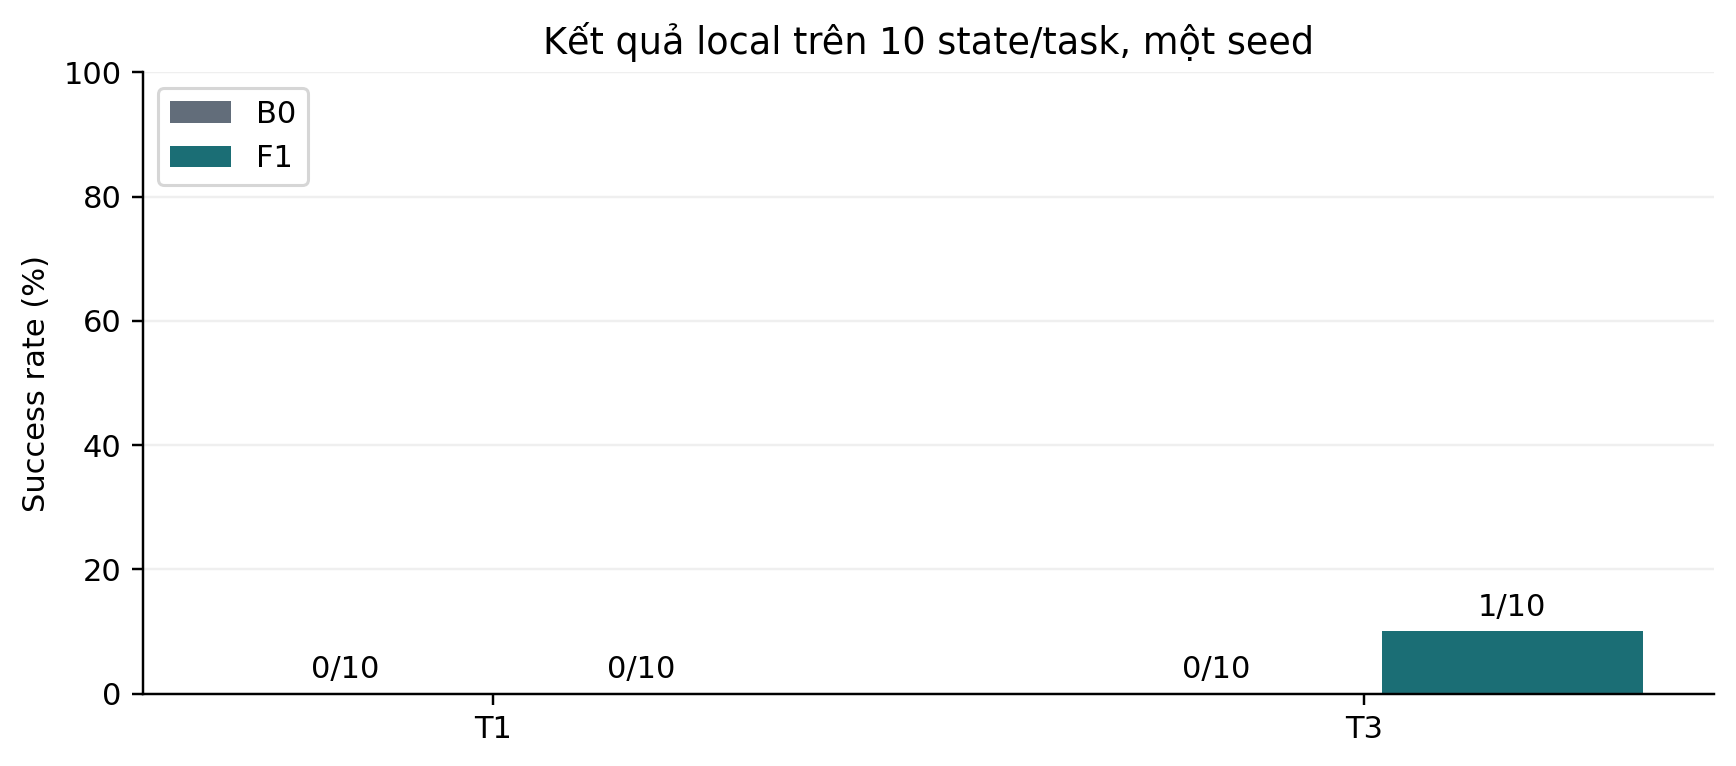
\includegraphics[width=\textwidth]{../figures/mem_success.png}
\caption{Tỷ lệ thành công trên T1 và T3 theo giao thức của khóa luận. Mỗi cột biểu diễn 10 quỹ đạo. Hai tác vụ dùng chung các nhóm trạng thái khởi tạo và cùng một hạt giống chính sách.}
\label{fig:mem_success}
\end{figure}

Gọi $S_{c,j}$ là chỉ báo thành công của điều kiện $c$ trên tổ hợp tác vụ và trạng thái thứ $j$. Chênh lệch tỷ lệ thành công quan sát được tính theo

\begin{equation}
\widehat{\Delta}_{\mathrm{SR}}
=\frac{1}{M}\sum_{j=1}^{M}\left(S_{F1,j}-S_{B0,j}\right),
\qquad M=20.
\end{equation}

Có 19 cặp có kết quả $(0,0)$ và một cặp có kết quả $(0,1)$ theo thứ tự $(B0,F1)$, nên $\widehat{\Delta}_{\mathrm{SR}}=0{,}05$, tức 5 điểm phần trăm. Toàn bộ chênh lệch đến từ một lần thực thi T3. Hai tác vụ chia sẻ 10 nhóm trạng thái và thí nghiệm chỉ dùng một hạt giống, nên báo cáo giới hạn ở thống kê mô tả. Việc ước lượng độ bất định cần thêm biến thiên qua trạng thái và hạt giống, đồng thời giữ cấu trúc ghép cặp.

SCR ghi nhận mức hoàn thành từng phần. Trên T1, cả B0 và F1 đều có một quỹ đạo đạt mốc tiến độ nhưng tiếp tục đến mức vượt số chu kỳ. Trên T3, SCR trung bình của F1 là 0,1667 trong khi của B0 bằng 0, cho thấy bộ đánh giá ghi nhận thêm tiến độ ở một số lần chạy. Diễn giải này bổ sung cho tỷ lệ thành công, vì tiến độ từng phần và hoàn thành ở điểm cuối là hai tiêu chí khác nhau. Đối chứng F0 thích ứng trên cùng dữ liệu nhưng không có bộ nhớ và phép đánh giá F1 khi thay đổi có kiểm soát đầu vào lịch sử vẫn cần thiết để trả lời RQ1.

\section{Bất đồng giữa tiến độ quan sát và tiến độ được chấm}

Khi chính sách tự sinh quỹ đạo, nó có thể đưa hệ thống đến những tình huống ít gặp trong dữ liệu thao tác mẫu. Trên 20 quỹ đạo F1, 19 trạng thái bộ nhớ cuối báo lịch sử chưa đầy đủ. Trong 1.927 lần gọi chính sách, 1.894 lời nhắc chứa hậu tố bộ nhớ và 1.738 lời nhắc chứa cụm \path{history incomplete}. Hai số đếm ở cấp lời nhắc lần lượt phản ánh tần suất cung cấp bộ nhớ và tần suất báo lịch sử chưa đầy đủ. Chúng là các phép đo lặp theo thời gian trên cùng quỹ đạo. Độ đúng của từng sự kiện đòi hỏi đối chiếu với nhãn độc lập.

Quỹ đạo T3 thành công duy nhất của F1 là một trường hợp chẩn đoán cho RQ2. Tại bước 1.000, bộ đánh giá ghi đủ ba chu kỳ, điều kiện cuối được thỏa mãn và số chu kỳ không bị vượt. Bộ ghi thị giác cuối chỉ xác nhận hai lần đặt lại và đánh dấu lịch sử chưa đầy đủ. Bất đồng này làm suy yếu cách giải thích rằng chính sách dừng khi bộ đếm thị giác ghi đủ ba chu kỳ. Kết quả vẫn tương thích với nhiều cơ chế, chẳng hạn sử dụng một phần bằng chứng lịch sử, phản ứng với quan sát hiện tại, hoặc hành vi đã thay đổi qua thích ứng trọng số.

Trong lượt T1 của F1 bị vượt số chu kỳ, bộ đánh giá ghi một mốc và SCR bằng 1, nhưng dừng quỹ đạo tại bước 266 do vượt số chu kỳ. Bộ ghi thị giác cuối ghi nhận 0 lần đặt lại và lịch sử chưa đầy đủ. B0 cũng có một quỹ đạo T1 vượt số chu kỳ, ở trạng thái 3 và bước 290. Những trường hợp này chỉ ra hai vấn đề khác nhau: hệ thống có thể thực hiện thao tác đạt mốc nhưng không duy trì đúng điểm cuối, và bộ ghi thị giác có thể thiếu bằng chứng để xác nhận mốc mà bộ đánh giá đã ghi nhận. Muốn quy nguyên nhân cần nhãn độc lập theo thời gian và can thiệp riêng lên nội dung bộ nhớ trong khi giữ các điều kiện còn lại ổn định.

\section{Hiệu lực của kết luận và thiết kế kiểm chứng tiếp theo}

Đối với RQ2, sự phù hợp trong sáu quỹ đạo mẫu cung cấp bằng chứng về tính khả thi của việc biểu diễn tiến độ bằng sự kiện thị giác. Dấu thời điểm khả dụng cho phép kiểm tra dữ kiện nào đã có thể đưa vào lời nhắc tại từng bước. Khoảng cách giữa kết quả ghép mốc trên quỹ đạo mẫu và tỷ lệ lịch sử chưa đầy đủ trên quỹ đạo F1 đặt ra giới hạn về tính đại diện của phép kiểm chẩn đoán. Một tập nhãn độc lập gồm cả tình huống thất bại, với quy tắc ghép và dung sai đặt trước, cho phép ước lượng riêng xác nhận sai, bỏ sót, độ trễ và tỷ lệ tình huống chưa xác định.

Đối với RQ1, cần giữ dữ liệu, phân hoạch, ngân sách huấn luyện và quy tắc chọn checkpoint giống nhau khi so F0 với F1. Phép thử can thiệp lúc suy luận cần có điều kiện chỉ dùng thông tin hiện tại và điều kiện có cùng định dạng nhưng thay đổi giá trị lịch sử. Hai phép so sánh trả lời các câu hỏi khác nhau: thích ứng với bộ nhớ có tạo lợi ích vòng kín hay không, và chính sách đã thích ứng nhạy thế nào với nội dung cụ thể của bộ nhớ. Một tập trạng thái xác nhận độc lập với phát triển và nhiều hạt giống sẽ cho phép ước lượng chênh lệch ghép cặp cùng độ bất định ở cấp nhóm trạng thái. Chỉ đổi hạt giống trên các trạng thái đã dùng để phát triển không tạo một tập xác nhận độc lập.

Về khả năng duy trì kỹ năng trong RQ3, đánh giá chính F1 trên các tác vụ cơ sở ghép cặp với B0 là cách đo trực tiếp mức duy trì. Nếu mục tiêu là kiểm tra tính không kém hơn, cần xác định trước biên suy giảm có thể chấp nhận được và cỡ mẫu đủ để diễn giải biên đó. Cơ chế chọn lại trọng số B0 cho tác vụ cơ sở chỉ đo chất lượng của một quy tắc định tuyến và không định lượng kỹ năng của F1.

Đối với RQ2, ưu tiên can thiệp vào những yếu tố có thể đổi giá trị hoặc thời điểm khả dụng của bằng chứng, gồm quy ước ảnh, độ trễ xác nhận và số hành động giữa hai lần gọi chính sách. Có thể dùng cùng một quỹ đạo để kiểm tra tác động riêng lên chất lượng quan sát trước khi thay đổi các yếu tố đó trong vòng kín. Cần báo cáo cả thời gian mô phỏng và thời gian thực đo trên phần cứng. Thiết kế như vậy gắn mỗi phép đo với một cơ chế sai lệch cụ thể, từ sai số của biểu diễn cho đến hạn chế về cách sử dụng biểu diễn trong điều khiển.


% Generated from THESIS_DRAFT.md.
\chapter{Kết luận}

\section{Thành quả đã đạt được}

Khóa luận đã xây dựng một hướng bổ sung bộ nhớ sự kiện thị giác cho SmolVLA trong tác vụ nhấc và đặt lại bát. Hệ thống liên kết detection với đĩa gốc, ghi nhận departure/return bằng máy trạng thái và đưa snapshot đã kiểm nguồn vào prompt. Các cơ chế thời điểm khả dụng, incomplete history và giới hạn token giúp biểu đạt rõ thông tin nào được sử dụng tại mỗi quyết định.

Một quy trình thích ứng action expert bằng LoRA đã được triển khai và tạo ra adapter sau 3.000 bước huấn luyện. Các file export được xác minh theo manifest. Đợt rollout B0/F1 trên T1/T3 đã tạo đủ artifact cho 40 task-episodes, cho phép đối chiếu kết quả với prompt và trạng thái memory. Đây là bằng chứng về việc phương pháp đã được đưa vào một hệ thống thực thi, vượt qua mức chỉ có kiến trúc đề xuất.

\section{Điều rút ra từ kết quả hiện tại}

Kết quả hiện tại chưa chứng minh mục tiêu nâng cao hiệu năng đã đạt. F1 có một success trong 20 task-episodes trong khi B0 không có success, nhưng phép so sánh còn gộp adaptation và memory, số nhóm state nhỏ và chỉ có một seed. Không có cơ sở chuyển các con số này thành một cải thiện chính thức trên LIBERO-Mem hoặc một kết luận tổng quát về memory cho VLA.

Một kết luận có căn cứ hơn là chất lượng và khả năng sử dụng thông tin memory phải được kiểm tra độc lập với loss huấn luyện. Hầu hết snapshot cuối của F1 báo lịch sử chưa đầy đủ; success duy nhất không đi kèm việc writer đếm đủ các chu kỳ được evaluator ghi nhận. Vì vậy, việc đã tạo prompt, đã giảm loss offline và đã có rollout thành công là ba bằng chứng khác nhau, không thể thay thế cho nhau trong lập luận về hiệu quả của phương pháp.

Giá trị học thuật hiện có nằm ở cách đặt và làm rõ bài toán, thiết kế biểu diễn sự kiện có truy vết, cùng những phép kiểm giúp tránh kết luận vượt bằng chứng. Giá trị này cần được đánh giá trong phạm vi một khóa luận xây dựng và khảo sát hệ thống; chưa phải chứng minh tính mới toàn cầu hay ưu thế so với các kiến trúc memory lớn.

\section{Hạn chế và hướng phát triển}

Các hạn chế chính là phạm vi một quan hệ bát–đĩa, thiếu đánh giá event fidelity, chưa có F0 matched và retention của adapter hiện tại, cùng khác biệt chưa được đóng hoàn toàn giữa dữ liệu tác giả và runtime local. Chuỗi tạo dữ liệu derived mới còn cần export thật và audit hoàn chỉnh trước khi được dùng cho kết luận huấn luyện mới.

Hướng tiếp theo là hoàn thiện chuỗi dữ liệu có version, xây dựng đối chứng thích ứng không memory trên cùng demonstration, đo chất lượng writer và thực hiện paired evaluation với phạm vi holdout được công bố rõ. Sau khi làm rõ giá trị của lịch sử trong bài toán hẹp, nghiên cứu mới có cơ sở mở rộng sang nhiều thực thể, nhiều backbone hoặc robot thật. Tóm tắt và kết luận cuối cùng sẽ được cập nhật theo kết quả thực nghiệm bổ sung, kể cả khi kết quả đó không xác nhận giả thuyết ban đầu.

\cleardoublepage
\phantomsection
\addcontentsline{toc}{chapter}{Tài liệu tham khảo}
\bibliographystyle{unsrt}
\bibliography{references}
\appendix
\chapter{Nguồn dữ liệu và chi tiết tái lập}
Các đường dẫn tính từ thư mục gốc \texttt{Thesis\_26}.
Tập bằng chứng ngày 12/11/2026 lưu tại \path{docs/thesis/evidence/snapshot.json}.
Tệp \path{input_hashes.json} cùng thư mục ghi mã SHA-256 của các nguồn đã đối chiếu.

\section{Cấu hình và bản ghi thực nghiệm}
Bản ghi đánh giá vòng kín được lưu tại
\begin{quote}\small
\path{experiments/evaluation/results_mem_2/step5_test_20261109-093744}
\end{quote}
Mỗi điều kiện có bản kê \path{run_manifest.json}, phân hoạch đã khóa
\path{split.lock.json} và tóm tắt từng lượt trong \path{episodes/*/summary.json}.
Phép tổng hợp đối chiếu trạng thái hoàn tất và SHA-256 với \path{status.json}.
Bản kê lưu thiết lập điều khiển, danh sách trạng thái khởi tạo, phiên bản mã và mô hình.

Bản ghi huấn luyện được lưu tại
\begin{quote}\small
\path{experiments/training/results_mem_2/mem-adapter-20261105-083543}
\end{quote}
Nguồn dùng để đối chiếu gồm \path{run_config.json}, \path{metrics.jsonl},
\path{checkpoint-003000/progress.json} và bản xuất trong \path{pretrained_model}.
Danh mục và phân hoạch dữ liệu nằm tại \path{experiments/training/results_mem_2/mem-adapter-v1}.
Mã băm của trọng số nền và HDF5 gốc được tham chiếu theo bản kê.

Mô phỏng chạy trong WSL với Python 3.8.20, robosuite 1.4.0, MuJoCo 3.2.3 và
NumPy 1.22.4. Suy luận trên Windows dùng Python 3.12.2, torch 2.6.0+cu124,
LeRobot 0.6.1, transformers 5.5.4 và PEFT 0.19.1.
Huấn luyện dùng torch 2.11.0+cu130, LeRobot 0.6.1, transformers 5.5.4,
PEFT 0.21.2 và accelerate 1.15.0. Phiên bản mô hình SmolVLA và nguồn tác vụ
LIBERO-Mem được ghi trong danh mục tài liệu tham khảo và trong bản kê từng lần chạy.

\section{Tệp dữ liệu phân tích và bối cảnh V1}
\path{docs/thesis/evidence/mem_test_episodes.csv} giữ một dòng cho mỗi
lượt, gồm kết quả, mã băm trạng thái, seed, tiến độ do bộ chấm và bộ ghi
xác định, cờ lịch sử và nguồn bản tóm tắt. \path{mem_test_counts.csv} tổng hợp
theo tác vụ. \path{validation_loss.csv} lấy từ nhật ký xác thực.
\path{historical_run_inventory.csv} là danh mục các lần chạy lịch sử.

Ở giai đoạn V1, báo cáo nội bộ ghi 77/160 lượt thành công trên 40 tác vụ,
28/40 trên tập nghiệm thu, và 11/40 trên LIBERO-10. Trong 83 lượt thất bại,
71 lượt chưa được quy nguyên nhân gốc theo tiêu chí chẩn đoán của báo cáo.
Tại mốc tổng hợp, các bản ghi từng lượt vắng mặt ở đường dẫn báo cáo dẫn chiếu.
Các số liệu này được dẫn theo báo cáo V1 và dùng làm bối cảnh lịch sử.
V1 dùng $s=50$ giữa hai lần truy vấn, còn đánh giá T1/T3 dùng $s=10$.
Khác biệt về nhịp điều khiển và tập tác vụ giới hạn khả năng đối chiếu giữa hai giai đoạn.

\section{Đối chiếu bản ghi sự kiện thị giác}
Phép đo ngày 26/10 được tổng hợp tại
\path{experiments/audits/memory_writer_v3/verification_summary.json}.
Nhãn tham chiếu đánh dấu mốc tiến độ tích lũy trên các quỹ đạo trình diễn.
Các báo cáo ghép mốc, kết quả thành phần và bản lưu mã nguồn được đối chiếu
SHA-256. Tập bằng chứng cũng ghi kết quả so khớp phiên bản của bộ theo dõi,
bộ ghi và bộ dựng văn bản với phiên bản dùng trong lần đo.

Các phép kiểm kỹ thuật đi kèm gồm đối chiếu đầu ra nhận dạng trên 12 khung hình,
đối chiếu chỉ mục trên 162 mẫu, 49 kiểm thử thành phần và 47 kiểm thử hồi quy.
Những phép kiểm này hỗ trợ đánh giá tính nhất quán của quy trình xử lý.
Độ phù hợp của sự kiện được phân tích bằng mốc chú giải và các quỹ đạo
trong Chương 4.

\section{Tái tổng hợp số liệu}
\path{docs/thesis/README.md} ghi các lệnh đọc bản ghi đã lưu, tổng hợp số liệu
và tái tạo tài liệu. Mỗi lần tổng hợp sử dụng tập bằng chứng và mã băm tương ứng.

\end{document}
